\chapter{Ασφάλεια}
\label{chapter:security}

Η κρυπτογραφία αναπτύσσεται επιδιώκοντας την ασφάλεια. Η επιφάνεια του αντικειμένου της ασφάλειας ενός κρυπτογραφικού σχήματος είναι πολύ ευρεία, ξεκινάει από την στιγμή που σχεδιάζεται αυτό και τελειώνει, ίσως, όταν αυτό αρχίσει να χρησιμοποιείται στην πράξη. Στο κεφάλαιο αυτό θα μελετήσουμε, από τις μόνες μορφές αποδείξιμης  ασφάλειας, την θεωρητική ασφάλεια ενός σχήματος. Επειδή, στα πλαίσια αυτής της εργασίας πραγματευόμαστε αποκλειστικά την θεωρητική ασφάλεια, θα αναφερόμαστε σε αυτήν απλά ως ασφάλεια. Προφανώς, ακόμα και η έννοια της θεωρητικής ασφάλειας ίσως να ακούγεται πολύ γενική. Παρατηρούμε ότι ανάλογα με την κατηγορία του σχήματος ή του εκάστοτε αλγορίθμου που εξετάζουμε επιθυμούμε να έχει και διαφορετικές ιδιότητες. Για παράδειγμα, με  διαφορετικό τρόπο ορίζουμε την ασφάλεια για ένα SMPC πρωτόκολλο και με διαφορετικό για ένα σχήμα δημόσιου κλειδιού, αφού διαθέτουν ποιοτική διαφορά. Επίσης, αν λάβουμε υπόψιν και την ισχυρότατα της ασφάλειας που επιθυμούμε να αποδείξουμε, μοντελοποιούμε και τον αντίπαλο του σχήματος με διαφορετικό τρόπο και άρα προκύπτει και μια ποσοτική διαφορά των ιδιοτήτων ασφάλειας. Αυτό συνήθως συμπεριλαμβάνει τους υπολογιστικούς πόρους και τις προθέσεις (π.χ. να γίνει αντιληπτός) που μπορεί να έχει κάποιος επιτιθέμενος για να σπάσει την ιδιότητα της ασφάλειας αλλά και το κέρδος που μπορεί να έχει από αυτό. Έτσι, για παράδειγμα, διαφορετικό τύπο αντιπάλων θα υποθέταμε στην μοντελοποίηση της ασφάλειας ενός κρυπτοσυστήματος ανταλλαγής κρατικών μυστικών και διαφορετικό τύπου αντιπάλων για ένα ανταλλαγής δεδομένων μεταξύ αισθητήρων που μετράνε το οξυγόνο σε ένα δάσος, υποθέτοντας ότι η πρόσβαση σε αυτά τα δεδομένα δεν δίνει κάποιο ιδιαίτερο κέρδος σε έναν αντίπαλο. Έτσι, ένα τυπικό παράδειγμα ισχυρισμού για την ασφάλεια ενός κρυπτοσυστήματος είναι το εξής :
"Σημασιολογικά ασφαλές για υπολογιστικά περιορισμένους αντιπάλους". Στο παράδειγμα αυτό, "Σημασιολογικά ασφαλές" είναι η ιδιότητα που επιθυμούμε να έχει το κρυπτοσύστημα μας και "Υπολογιστικά περιορισμένοι αντίπαλοι", είναι ως προς ποιο μοντέλο αντιπάλων επιθυμούμε να ισχύει αυτή η ιδιότητα. Όμως δεν αρκεί απλά να ισχυριστούμε ότι ένας αλγόριθμος είναι ασφαλείς πρέπει και να το αποδείξουμε. Στην συνέχεια του κεφαλαίου θα παρουσιαστούν και θα μελετηθούν βασικοί ορισμοί μοντέλων αντιπάλων, βασικοί ορισμοί της ασφάλειας, τυπικών ισχυρισμών αυτής, μεθόδων απόδειξης και βασικών μοντέλων/υποθέσεων στα οποία ανάγουμε αυτές. Πριν ξεκινήσουμε την μελέτη μας πρέπει πρώτα να δώσουμε έναν γενικό ορισμό ενός αντιπάλου τον οποίο θα κάνουμε πιο συγκεκριμένο στην συνέχεια του κεφαλαίου. Αυτός είναι ο εξής :

\begin{definition}
\textbf{Αντίπαλος κρυπτογραφικού σχήματος} : Είναι μια οντότητα ο οποία μπορεί να "χειρίζεται" έναν ή και περισσότερους συμμετέχοντες (ανάλογα με το πόσοι συμμετέχουν στο κρυπτογραφικό σχήμα) σε σχήμα, δηλαδή μπορεί να διαφθείρει έναν ή περισσότερους συμμετέχοντες με σκοπό να λειτουργήσουν σύμφωνα με το δικό του σκοπό. Στην πράξη μοντελοποιείται με έναν αλγόριθμο ή που ελέγχει όλους τους διεφθαρμένους συμμετέχοντες. Προφανώς, δεν έχει νόημα να θεωρήσουμε έναν αντίπαλο που ελέγχει όλους τους συμμετέχοντες ενός σχήματος.
\end{definition}

Στο σημείο αυτό πρέπει να αναφέρουμε ότι για πολλούς από τους ορισμούς που θα μελετήσουμε έχουν χρησιμοποιηθεί ως βιβλιογραφικές πηγές οι \cite{Bauer2011}, \cite{hoffstein2008introduction}, \cite{10.1561/3300000019}.

\section{Βασικοί Ορισμοί}

Στην ενότητα αυτή θα γίνει μια εισαγωγή στην βασική σημειολογία της θεωρητικής ασφάλειας, στα βασικά μοντέλα ασφάλειας και στις βασικές κρυπτογραφικές υποθέσεις που χρησιμοποιούμε για να καταφέρουμε να αποδείξουμε την ασφάλεια ενός κρυπτογραφικού σχήματος.
\subsection{Βασική Σημειολογία}

Θα ξεκινήσουμε με μια εισαγωγή στην σημειολογία που χρησιμοποιείται στην θεωρητική ασφάλεια. Δεν μπορούμε να ξεκινήσουμε παρά ορίζοντας μια συνάρτηση που είναι πανταχού παρόν στην κρυπτογραφία και κυρίως στις αποδείξεις υπολογιστικής ασφάλειας. Αυτή της μηδαμινής συνάρτησης, που ορίζεται ως εξής :

\begin{definition}
\textbf{Μηδαμινή συνάρτηση (Negligible function)} : Κάθε συνάρτηση $negl: \mathbb{N} \rightarrow \mathbb{R}$ που συναρτήσει της εισόδου της $Ν$, τείνει ως προς το $0$ ασυμπτωτικά γρηγορότερα από κάθε αντίστροφη θετική πολυωνυμική συνάρτηση.
\end{definition}

Συνήθως στις αποδείξεις ασφάλειας η μηδαμινή συνάρτηση παίρνει ως είσοδο κάποια παράμετρο ασφάλειας, οπότε στη βιβλιογραφία πολύ συχνά συναντάμε συμβολισμούς όπως ο $negl(\secparam)$. Πολύ βασική είναι επίσης και η έννοια της δυσδιακριτότητας μεταξύ δύο κατανομών, διακρίνουμε δύο τύπους δυσδιακριτότητας ανάλογα με τους υπολογιστικούς πόρους το αντιπάλου, την υπολογιστική και την στατιστική, που ορίζονται ως εξής :

Έστω ότι έχουμε δύο πιθανοτικούς αλγορίθμους, που η έξοδος του ακολουθεί κατανομή $D_1$ και $D_2$ αντίστοιχα.

\begin{definition}
\textbf{Στατιστική δυσδιακριτότητα (Statistical Indistinguishability)} : Οι κατανομές $D_1$ και $D_2$ έχουν Στατιστική δυσδιακριτότητα (Indistinguishable distributions), αν για οποιονδήποτε αλγόριθμο (ακόμα και με απεριόριστους υπολογιστικούς πόρους) $A$ ισχύει:
$$
\operatorname{Pr}\left[A(D_{1}(n))=1\right]-\operatorname{Pr}\left[A(D_{2}(n))=1\right] \leq negl(\secparam)
$$
όπου $Δ$ είναι η στατιστική απόσταση των δύο κατανομών, όπου $n$ μια παράμετρος ασφάλειας. 
\end{definition}

\begin{definition}
\textbf{Υπολογιστική Δυσδιακριτότητα (\EN{Computational Indistinguishability})} : Οι κατανομές $D_1$ και $D_2$ έχουν Υπολογιστική δυσδιακριτότητα (Computational indistinguishability), αν για οποιονδήποτε μη ομοιόμορφο πιθανοτικό πολυωνυμικό αλγόριθμο (non-uniform PPT) $A$ ισχύει:
$$
\operatorname{Pr}\left[A(D_{1}(n))=1\right]-\operatorname{Pr}\left[A(D_{2}(n))=1\right] \leq negl(\secparam)
$$
όπου $n$ μια παράμετρος ασφάλειας.
\end{definition}

Οι έννοιες τις δυσδιακριτότητας είναι ιδιαίτερα χρήσιμες στις αποδείξεις ασφάλειας καθώς ο στόχος κάθε απόδειξης είναι να δείξουμε ότι η κατανομή των δεδομένων που γνωρίζει ένας αντίπαλος μέσω κάποιου κρυπτογραφικού σχήματος είναι δυσδιάκριτη από κάποια τυχαία κατανομή.
Οι παράμετροι ασφάλειας (security parameters) εμφανίζονται στις αποδείξεις ασφάλειας κρυπτογραφικών σχημάτων ως ένας τρόπος ποσοτικοποίησης της ασφάλειας, δηλαδή της δυσκολίας του αντιπάλου να σπάσει την ασφάλεια τους. Ουσιαστικά οι παραμέτροι ασφάλειας είναι ένα μέτρο ποσοτικοποίησης του πλεονεκτήματος του αντιπάλου σε ένα σύστημα. Όπως θα δούμε και στη συνέχεια, είναι άμεσα συσχετισμένο με τις έννοιες τις δυσδιακριτότητας. Στην βιβλιογραφία απαντάμε δύο κύριες παραμέτρους ασφάλειας, αυτή της στατιστικής και αυτή της υπολογιστικής.
 
Η παράμετρος της υπολογιστικής ασφάλειας προφανώς σχετίζεται με την Υπολογιστική Ασφάλεια και άρα με την ποσοτικοποίηση της δυσκολία επίλυσης κάποιου υπολογιστικού προβλήματος από έναν υπολογιστικά περιορισμένο αντίπαλο. Ας δούμε ένα πρακτικό παράδειγμα. Σε ένα πρωτόκολλο RSA για παράδειγμα η παράμετρος υπολογιστικής ασφάλειας είναι είσοδος της συνάρτησης $\kgen$, αφού πρόκειται και πρακτικά είναι το μήκος $\secpar$ σε bit των πρώτων αριθμών $p$,$q$ που επιλέγουμε τέτοιοι ώστε $N=p \cdot q$. Είναι σύνηθες να απαντάμε αυτή την παράμετρο ως το μήκος κλειδιού που χρησιμοποιείται σε ένα σχήμα. Την ορίζουμε ως εξής :

\begin{definition}
\textbf{Παράμετρος υπολογιστικής ασφάλειας (\EN{Computational security parameter}) $\secpar$} : Είναι η παράμετρος που σχετίζεται με την δυσκολία σπασίματος προβλημάτων από τον αντίπαλο μέσω της υπολογιστικής ισχύς του. Όταν δίνεται ως όρισμα σε μια συνάρτηση συμβολίζεται με τον μοναδιαίο συμβολισμό $\secparam$.
\end{definition}

Αντίστοιχα, η παράμετρος της στατιστικής ασφάλειας σχετίζεται με την Στατιστική Ασφάλεια, δηλαδή με την ποσοτικοποίηση της δυσκολίας επίλυσης κάποιου προβλήματος, με την γενικότερη έννοια, που δεν σχετίζεται με την υπολογιστική ισχύ του αντιπάλου, αφού στην περίπτωση της Στατιστικής Ασφάλειας υποθέτουμε ότι ο αντίπαλος διαθέτει άπειρους υπολογιστικούς πόρους. Για παράδειγμα, σε ένα διαδραστικό πρωτόκολλο ο αντίπαλος μπορεί να διαθέτει μια μοναδική ευκαιρία να παραβιάσει την ασφάλεια του πρωτοκόλλου αν καταφέρει να προβλέψει μια τυχαία τιμή που θα επιλέξει ο 
κάποιος συμμετέχον στον επόμενο γύρο. Είναι προφανές ότι πρόβλεψη αυτής της τιμής είναι ανεξάρτητη από τους υπολογιστικούς πόρους του αντιπάλου. Την πιθανότητα να προβλέψει αυτή την τιμή την ποσοτικοποιούμε με την παράμετρο αυτή. Η παράμετρος ορίζεται ως εξής :

\begin{definition}
\textbf{Παράμετρος στατιστικής ασφάλειας (\EN{Statistical security parameter}) $σ$} : Είναι η παράμετρος που σχετίζεται με την δυσκολία σπασίματος προβλημάτων που δεν σχετίζονται με την υπολογιστική του ισχύ αντιπάλου. Όταν δίνεται ως όρισμα σε μια συνάρτηση συμβολίζεται επίσης με τον μοναδιαίο συμβολισμό $1^σ$.
\end{definition}

Πρέπει να αναφέρουμε πως εκ των ονομάτων των παραμέτρων αυτών, είναι απολύτως λογικό να περίμενε κάποιος σε ένα κρυπτογραφικό σχήμα να υπάρχει μια παράμετρος ασφαλείας η οποία ανάλογα με το τι είδος ασφάλειας θέλουμε να αποδείξουμε να ονομάζεται στατιστική ή υπολογιστική παράμετρος ασφάλειας αντίστοιχα. Η αλήθεια είναι ότι σε πιο σύνθετα σχήματα, όπως για παράδειγμα το πρωτόκολλο Cut-and-Choose που θα δούμε στο Κεφάλαιο \ref{chapter:SMPC}, μπορούν να περιέχουν και τις δύο παραμέτρους ασφάλειας. Στην περίπτωση αυτή ο σωστός τρόπος να ερμηνεύσουμε την ασφάλεια του συστήματος είναι ως : $2^{-σ} + negl(\secparam)$. Είναι προφανές ότι στην περίπτωση που υπάρχουν και οι δύο παράμετροι ασφαλείας το μέγιστο επίπεδο ασφάλειας που μπορεί να επιτύχει ένα σχήμα είναι αυτό της Υπολογιστικής Ασφάλειας.

\subsection{Βασικά Κρυπτογραφικά Μοντέλα}

Θα συνεχίσουμε με τα βασικά κρυπτογραφικά μοντέλα ή αφαιρέσεις που χρησιμοποιούνται στην θεωρητική ασφάλεια. Η απόδειξη της θεωρητικής ασφάλειας ενός κρυπτογραφικού σχήματος δεν είναι καθόλου εύκολη υπόθεση. Πολλές φορές για να γίνει εφικτή η απόδειξη αυτή χρειάζεται να μοντελοποιήσουμε ή να εξιδανικεύσουμε αρκετά στοιχεία του σχήματος που εξετάζουμε, όπως για παράδειγμα στοιχεία που σχετίζονται με την υλοποίηση ή στοιχεία που σχετίζονται με κρυπτογραφικά εργαλεία που χρησιμοποιεί το σχήμα τα οποία τα θεωρούμε ως ιδανικά ώστε να διαχωρίσουμε τις αποδείξεις ασφάλειας του. Για παράδειγμα, μια συνάρτηση κατακερματισμού μπορούμε να την μοντελοποιήσουμε ως ένα Τυχαίο Μαντείο όταν χρησιμοποιείται ως συστατικό στοιχεία σε ένα σχήμα. Η εξέταση του κατά πόσο η συνάρτηση αυτή προσεγγίζει το μοντέλο αυτό αποτελεί αντικείμενο κάποιας άλλης απόδειξης. Ας ξεκινήσουμε με το πιο απλό αλλά και ταυτόχρονα το πιο ισχυρό μοντέλο ασφάλειας. Στο μοντέλο αυτό θεωρείται εξαιρετικά δύσκολο να αποδειχθεί κάποιο σχήμα ότι είναι ασφαλές. 

\begin{definition}
\textbf{Κανονικό Μοντέλο (Standard Model ή SM)} : Στο μοντέλο αυτό o μόνος περιορισμός ενός επιτιθέμενου είναι ότι διαθέτει υπολογιστικά περιορισμένους πόρους και ότι ισχύουν οι συνήθεις εικασίες πολυπλοκότητας συγκεκριμένων προβλημάτων και κλάσεων προβλημάτων, όπως για παράδειγμα για το DLP ή για την παραγοντοποίηση σε πρώτους παράγοντες.
\end{definition}

Στο μοντέλο αυτό, δεν είναι καθόλου πρακτικό καθώς κάνει τις ελάχιστες δυνατές υποθέσεις. Πολλά πρωτόκολλα που έχουν προταθεί ως ασφαλή στο μοντέλο αυτό εν τέλει έχουν απορριφθεί λόγω του ότι βρέθηκαν λάθη στην απόδειξη της ασφάλειας τους.

Το επόμενο μοντέλο που θα μελετήσουμε κάνει μια σχετικά απλή υπόθεση, μια εξιδανίκευση της υλοποίησης. Ας το δούμε πρώτα μέσα από ένα παράδειγμα. Ένα κρυπτογραφικό σχήμα, όπως το Diffie-Hellman γνωρίζουμε ότι χρησιμοποιεί μια πεπερασμένη πολλαπλασιαστική ομάδα μεγάλης πρώτης τάξης. Η υλοποιητική αναπαράσταση της ομάδας αυτής μπορεί να φανερώνει πληροφορίες σχετικά με την εσωτερική δομή της, γεγονός που να επιτρέπει την χρήση πιο εξειδικευμένων και γρήγορων αλγορίθμων, σε σχέση με γενικευμένους αλγόριθμους (π.χ. γενικευμένους αλγορίθμους αναζήτησης όπως ο Baby step-Giant), για την επίλυση του DLP ή του CDH προβλήματος. Επιθέσεις που σχετίζονται με την εκάστοτε υλοποίηση κάποιου σχήματος δεν μπορούμε να της λάβουμε υπόψη, αφού αντικείμενο της θεωρητικής ασφάλειας δεν είναι η υλοποίηση ενός αλγορίθμου παρά μόνο ο αλγόριθμος ενός σχήματος. Έτσι το 1997 προτάθηκε από τον Shoup στην εργασία \cite{shoup1997lower} ένα μοντέλο για την επίλυση αυτού του προβλήματος, δηλαδή την μοντελοποίηση της υλοποίησης μιας αλγεβρικής ομάδας.

\begin{definition}
\textbf{Μοντέλο Γενικευμένης Ομάδας (\EN{Generic Group Model ή GGM}) \cite{cryptoeprint:2006/230}} : Έστω μια πολλαπλασιαστική ομάδα $\langle G, \cdot \rangle$, με $ord(G)=q$ και μια συνάρτηση κωδικοποίησης $σ : \mathcal{Z} \rightarrow {0,1}*$. Στο μοντέλο αυτό οποιαδήποτε αλληλεπίδραση με στοιχεία της ομάδας γίνεται μόνο μέσω ενός μαντείου $\oracle$. Το μαντείο αυτό υποστηρίζει δύο είδους ερωτήματα :
\begin{itemize}
    \item $\oracle(i)$, με $i \in [0, q]$ : Επιστρέφει $σ(i)$. Αν δεν έχει ξανά δεχτεί το ίδιο ερώτημα $i$ επιστρέφει μια ομοιόμορφα τυχαία τιμή διαφορετικά επιστρέφει την ίδια τιμή $σ(i)$ που επέστρεψε και στο παρελθόν.
    \item $\oracle(r, s, σ(i), σ(j))$, με $r, s \in [0, q]$ : Επιστρέφει $σ(ri + sj \mod q)$. Ψάχνει τα  $σ(i)$ και  $σ(j)$ στον κατάλογο του, βρίσκει τα αντίστοιχα $i$, $j$ και υπολογίζει την τιμή $k=ri+sj modq$. Στην συνέχεια εκτελεί το $\oracle(k)$.
\end{itemize}
\end{definition}

Μπορεί παρόμοια να οριστεί και Γενικευμένο Μοντέλο Δακτυλίων. Το παραπάνω μοντέλο θεωρείται αρκετά εξιδανικευμένο αφού για παράδειγμα σε πολλές υλοποιήσεις το ταυτοτικό στοιχείο αναπαρίσταται με το 1, το οποίο έρχεται σε πλήρη αντίθεση με το μοντέλο GGM. Το μοντέλο αυτό έχει δεχτεί αρκετή κριτική από την βιβλιογραφία κυρίως γιατί έχουν υπάρξει παραδείγματα αποδείξεων για κρυπτογραφικά σχήματα, όπως η \cite{bellare1994optimal} για το σχήμα RSA-OAEP, οι οποίες βασίζονταν το GGM και εν τέλη αποδείχθηκε ότι διέθεταν λάθος στην απόδειξη, όπως η \cite{nguyen2001insecurity} για το RSA-OAEP. Ωστόσο, συνήθως τα προβλήματα στις αποδείξεις αυτές όπως αναλύεται στην εργασία \cite{cryptoeprint:2006/230} δεν σχετίζονται άμεσα με το GGM αλλά με το ότι μπορεί να απλοποιήσει σημαντικά τις διαδικασίες απόδειξης με αποτέλεσμα να παραληφθούν άλλες σημαντικές επιφάνειες επίθεσης στην ασφάλεια ενός σχήματος.

Ένα ακόμα μοντέλο που χρησιμοποιείται ευρέως είναι αυτό του Τυχαίου Μαντείου. Συνήθως χρησιμοποιείται ως αφαίρεση για μια κρυπτογραφική συνάρτηση κατακερματισμού που μπορεί να χρησιμοποιεί κάποιο σχήμα. Όπως και το GGM, στην βιβλιογραφία θεωρείται ως αρκετά ουτοπικό καθώς αρκετές συναρτήσεις κατακερματισμού που χρησιμοποιούνταν σε κρυπτογραφικές υλοποιήσεις έως και πριν μερικά χρόνια, όπως η SHA-1 ή η MD5, δεν μπορούν να μοντελοποιηθούν σωστά από αυτό το το μοντέλο αυτό, αφού είναι γνωστό πως είναι ευάλωτες σε Επιθέσεις Επέκτασης Μήκους. Το μοντέλο αυτό ορίζεται ως εξής :

\begin{definition}
\textbf{Μοντέλο Τυχαίου Μαντείου (Random Oracle Model ή ROM)} : Πρόκειται για ένα μαντείο $\oracle \rightarrow {0,1}^* \times {0,1}^*$ που δέχεται ερωτήματα με μια παράμετρο, δηλαδή $\oracle(i)$ και επιστρέφει μια τιμή. Αν η τιμή $i$ δεν έχει επαναληφθεί σε προηγούμενο ερώτημα τότε η τιμή που επιστρέφεται είναι μια ομοιόμορφα τυχαία τιμή. Διαφορετικά αν η τιμή $i$ έχει επαναληφθεί επιστρέφεται τιμή που είχε επιστραφεί στο τελευταίο ερώτημα για την τιμή $i$ 
\end{definition}

Έχει αποδειχθεί ότι δεν μπορούμε να κατασκευάσουμε συναρτήσεις που να έχουν τις ιδιότητες ενός Τυχαίου Μαντείου και ταυτόχρονα να είναι υπολογιστικά αποδοτικές. Αυτό έχει ως αποτέλεσμα πολλά κρυπτογραφικά σχήματα να χρησιμοποιούν κρυπτογραφικές συναρτήσεις, οι οποίες είναι αποτελεσματικές με τα όποια όμως μειονεκτήματα υπάρχουν σε αυτές και στην συνέχεια να αφήνεται στην επιστημονική κοινότητα να καταλήξει στο αν αυτά τα μειονεκτήματα μπορούν να χρησιμοποιηθούν αποτελεσματικά για την παραβίαση της ασφάλειας του σχήματος.

Σε πολλά μη διαδραστικά σχήματα, όπως οι Μη Διαδραστικές Αποδείξεις Μηδενικής Γνώσης που θα εξετάσουμε σε επόμενη ενότητα, προκειμένου να απλοποιηθεί η απόδειξη του σχήματος χρειάζεται να υποθέσουμε κάποιο κοινό σημείο εκκίνησης, κάποια κοινή γνώση μεταξύ των συμμετεχόντων. Η πληροφορία αυτή συνήθως διατυπώνεται με την μορφή συμβολοσειρών αλλά μπορεί να έχει και οποιαδήποτε άλλη μορφή, δηλαδή ότι οι συμμετέχοντες έχουν όλοι στην κατοχή τους την ίδια συμβολοσειρά. Αυτή την συμβολοσειρά μπορεί να έχουν χρησιμοποιήσει κάποιο άλλο πρωτόκολλο για να την αποκτήσουν είτε απλά να βασιστούν σε έναν έμπιστο τρίτο άτομο να την διαμοιράσει σε αυτούς. Έτσι προκύπτει το παρακάτω μοντέλο.

\begin{definition}
\textbf{Μοντέλο Συμβολοσειρών Κοινής Αναφοράς (\EN{Common Reference String Model} ή CRSM)} : Το μοντέλο μοντέλο αυτό υποθέτει ότι όλες οι οντότητες ενός κρυπτογραφικού σχήματος έχουν πρόσβαση σε μια συμβολοσειρά $crs$ που ανήκει σε μια προκαθορισμένη κατανομή $D$.
\end{definition}

\subsection{Βασικές Κρυπτογραφικές Υποθέσεις}

Τελειώνοντας με την μελέτη της σημειολογίας στις αποδείξεις θεωρητικής ασφάλειας, δεν μπορούμε να παραλείψουμε τις βασικές κρυπτογραφικές υποθέσεις ή καλύτερα βασικές υποθέσεις της υπολογιστικής πολυπλοκότητας που έχουν εφαρμογή στην κρυπτογραφία. Αυτές πρόκειται για προτάσεις που δεν έχουμε καταφέρει να αποδείξουμε ούτε ότι ισχύουν αλλά ούτε το αντίθετο. Ωστόσο, τα περισσότερα κρυπτογραφικά σχήματα που έχουν αναφερθεί στην κρυπτογραφία βασίζουν την ασφάλεια τους σε αυτές τις υποθέσεις. Για παράδειγμα, ο κλάδος της κρυπτογραφίας δεν έχει καταφέρει να αποδείξει αν το πρωτόκολλο ανταλλαγής κλειδιών Diffie-Hellman είναι υπολογιστικά ασφαλές στο κλασσικό μοντέλο υπολογισμού (στο κβαντικό μοντέλο υπολογισμού γνωρίζουμε ότι δεν είναι), ωστόσο επειδή έχουν περάσει σχεδόν 50 χρόνια από τότε που προτάθηκε εικάζεται στην βιβλιογραφία ότι είναι πολύ πιθανό αυτό να συμβαίνει. Έτσι επειδή και άλλα σχήματα βασίζονται στο ίδιο πρόβλημα με αυτό του Diffie-Hellman, έχουμε δημιουργήσει ένα πρόβλημα για αυτό, αλλά και μια συσχετιζόμενη υπόθεση με το πρόβλημα αυτό. Το πρόβλημα Diffie-Hellman το απαντάμε σε δύο παραλλαγές αυτή του Υπολογιστικού και αυτή του Αποφαστιστικού Προβλήματος Diffie Hellman. Προφανώς υπάρχουν και οι αντίστοιχες υποθέσεις. Αυτές είναι οι παρακάτω.

\begin{definition}
\textbf{Υπόθεση Αποφαστιστικού Diffie-Hellman (\EN{Decisional Diffie-Hellman} ή \EN{DDH Assumption})} :
Έστω μια πολλαπλασιαστική ομάδα πρώτης τάξης $G$. Η DDH υπόθεση εκφράζει ότι οι πιθανοτικές κατανομές $(g^{a},g^{b},g^{ab})$ και $(g^{a},g^{b},g^{c})$, όπου $a, b, c \in G$ είναι τυχαία και ομοιόμορφα επιλεγμένα, είναι υπολογιστικά δυσδιάκριτες. Ισοδύναμα, το πλεονέκτημα οποιοδήποτε μη ντετερμινιστικού αντιπάλου με υπολογιστικά περιορισμένους πόρους που προσπαθεί να τις διακρίνει είναι το πολύ μηδαμινό σε συνάρτηση της παραμέτρου ασφάλειας η οποία είναι ο αριθμός των ψηφίων της τάξης της ομάδας $G$. Πιο αυστηρά το ορίζουμε το εξής :
$$
\forall A \in PPT : Pr[A(g^a, g^b, g^ab) = 1] - Pr[A(g^a, g^b, g^c)] \le negl(\secparam) = ε_{DDH}
$$
όπου $a, b, c \sample G$
Το πλεονέκτημα το συμβολίζουμε με $ε_{DDH}$.
\end{definition}

\begin{definition}
\textbf{Υπόθεση Υπολογιστικού Diffie-Hellman (\EN{Computational Diffie-Hellman} ή \EN{CDH Assumption})} :
Έστω μια πολλαπλασιαστική ομάδα πρώτης τάξης $G$. Η CDH υπόθεση εκφράζει ότι οποιοσδήποτε πολυωνυμικός αλγόριθμος με είσοδο την τριάδα $(g^{a},g^{b}, g)$ όπου $a, b, g \in G$ είναι τυχαία και ομοιόμορφα επιλεγμένα έχει το πολύ μηδαμινή πιθανότητα εύρεσης του $g^{ab}$.
\end{definition}

Είναι πολύ εύκολο να αποδειχθεί ότι η υπόθεση DDH είναι πιο ισχυρή υπόθεση από την CDH. Για λόγους πληρότητας αναφέρουμε πως το DHKE βασίζεται στην CDH υπόθεση, ωστόσο η DDH ονομάστηκε έτσι γιατί είναι συγγενικά παρόμοια με αυτή της CDH. Μια ακόμα πολύ γνωστή υπόθεση που σχετίζεται με αυτές είναι η Υπόθεση Διακριτού Λογαρίθμου η οποία είναι πιο χαλαρή υπόθεση ακόμα και από το CDH. 

\begin{definition}
\textbf{Υπόθεση Διακριτού Λογαρίθμου (Discrete Logarithm Assumption)} : Έστω μια κυκλική πολλαπλασιαστική ομάδα $\langle G, \cdot \rangle$  με $G = \langle g \rangle$ όπου $g$ ένας γεννήτορας της $G$ (π.χ. η $\langle \mathbb{Z}_p, \cdot \rangle$ όπου  $p$ πρώτος αριθμός). Η υπόθεση αυτή εκφράζει ότι, οποιοσδήποτε πολυωνυμικός στον αριθμό ψηφίων της τάξης της ομάδας αλγόριθμος, για ένα τυχαίο στοιχείο $a \in G$ έχει μηδαμινή πιθανότητα επίλυσης του Προβλήματος Διακριτού Λογαρίθμου, δηλαδή την εύρεση $x \in G$ τέτοιου ώστε $log_g(a) = x$.
\end{definition}

\begin{definition}
\textbf{Υπόθεση Συνάρτηση Μονής Διαδρομής (One Way Function ή OWF)} : Μια συνάρτηση  $f : \bin^{*} → \bin^{*}$ η οποία είναι εύκολο να υπολογιστεί από έναν πολυωνυμικό στο χρόνο αλγόριθμο αλλά η αντίστροφη της, $f^{-1}$, δεν μπορεί να υπολογιστεί επιτυχώς με μη μηδαμινή πιθανότητα από οποιονδήποτε πολυωνυμικό αλγόριθμο.
\end{definition}

\section{Μοντέλα αντιπάλων}

Αφού είδαμε βασικούς ορισμούς της θεωρητικής ασφάλειας βασιζόμενοι στον γενικό ορισμό ενός κρυπτογραφικού αντιπάλου τώρα θα προχωρήσουμε στην εξειδίκευση αυτού του ορισμού. Είναι προφανές ότι για να δημιουργήσουμε την απόδειξη ασφάλειας ενός κρυπτογραφικού σχήματος είναι απαραίτητο να διαθέτουμε ένα μοντέλο του αντιπάλου που θα κληθεί αυτό να αντιμετωπίσει όταν υλοποιηθεί στην πράξη. Είναι πολύ σημαντική η επιλογή κατάλληλου αντιπάλου που να προσεγγίζει όσο πιο ρεαλιστικά γίνεται μια οντότητα που θα προσπαθήσει να παραβιάσει την ασφάλεια του σχήματος μας και πολλές φορές καθορίζει την πρακτικότητα του σχήματος μας. Στην βιβλιογραφία υπάρχουν διάφορες κατηγορίες με μοντέλα αντιπάλων τα οποία μπορούμε να χρησιμοποιήσουμε και να συνδυάσουμε ανάλογα με την φύση του εκάστοτε κρυπτογραφικού σχήματος και των ιδιοτήτων ασφάλειας που επιθυμούμε να αποδείξουμε. Παρακάτω αναφέρουμε τις βασικές κατηγορίες αντιπάλων που απαντώνται στη βιβλιογραφία και σε ποια χαρακτηριστικά βασίζεται η διαφοροποίηση τους:

\begin{definition}
\textbf{Κατηγορίες αντιπάλων}:
\begin{itemize}
    \item Αντίπαλοι διαφοροποιημένοι ως προς την υπολογιστική τους ισχύ.
    \item Αντίπαλοι διαφοροποιημένοι ως προς την δυνατότητα διαφθοράς των συμμετεχόντων.
    \item Αντίπαλοι διαφοροποιημένοι ως προς το πότε επιλέγονται οι διεφθαρμένοι συμμετέχοντες.
\end{itemize}
\end{definition}

Στην συνέχεια, αναλύουμε τις παραπάνω κατηγορίες. Προφανώς, ένας αντίπαλος μπορεί να συνδυάζει περισσότερα από ένα χαρακτηριστικά, τα οποία όμως ανήκουν σε διαφορετικές κατηγορίες.

\subsection{Αντίπαλοι διαφοροποιημένοι ως προς την υπολογιστική ισχύ}

Η διαφοροποίηση των αντιπάλων ως προς την υπολογιστική του ισχύ είναι αντίστοιχη με αυτήν την ύπαρξης δύο διαφορετικών παραμέτρων ασφαλείας που αναλύσαμε σε προηγούμενη ενότητα. Ως επί το πλείστον βέβαια τα κρυπτογραφικά σχήματα σήμερα προκειμένου να είναι πρακτικά είναι ασφαλή μόνο ενάντια σε υπολογιστικά φραγμένους αντιπάλους.

\begin{definition}
\textbf{Αντίπαλος με υπολογιστικά άπειρους πόρους (\EN{Computationally unbounded resources adversary})} είναι ένας αλγόριθμος, πιθανοκρατικός ή μη, ο οποίος έχει άπειρη υπολογιστική ισχύ.
\end{definition}

\begin{definition}
\textbf{Αντίπαλος με υπολογιστικά φραγμένους πόρους (\EN{Computationally bounded resources adversary})} είναι ένας πολυωνυμικός αλγόριθμος, πιθανοκρατικός ή μη, που τρέχει σε πολυωνυμικό χρόνο ως προς την παράμετρο υπολογιστική ασφάλειας $\secpar$.
\end{definition}

\subsection{Αντίπαλοι διαφοροποιημένοι ως προς την δυνατότητα διαφθοράς των συμμετεχόντων}

Η διαφοροποίηση αυτή τον αντίπαλων είναι αρκετά κρίσιμη και καθορίζει άμεσα τη χρησιμότητα του κρυπτογραφικού σχήματος αλλά και την δυσκολία απόδειξης της ασφάλειας του. Είναι προφανές ότι η μεγαλύτερη ισοδυναμεί με δυσκολότερη ή και αδύνατη την απόδειξη της ασφάλειας ενός κρυπτογραφικού σχήματος ενάντια σε έναν τέτοιο αντίπαλο. Οι κύριες κατηγορίες αντιπάλων ως προς την δυνατότητα διαφθοράς των συμμετεχόντων σε ένα κρυπτογραφικών σχήμα είναι οι παρακάτω :

\begin{definition}
\textbf{Παθητικός αντίπαλος (\EN{Passive adversary}) ή Περίεργος αντίπαλος (\EN{Honest-but-curious adversary})} είναι ένας αλγόριθμος, πιθανοκρατικός ο οποίος δεν επεμβαίνει παρεμβατικά στο κρυπτοσύστημα με τρόπο ώστε να αλλάξει τον τρόπο εκτέλεσης του. Εκτελεί το κρυπτοσύστημα σωστά, ωστόσο από τις πληροφορίες που συλλέγει, από τους συμμετέχοντες που έχει διαφθείρει, μπορεί να εκτελέσει επιπλέον υπολογισμούς με σκοπό την εξαγωγή επιπλέον πληροφοριών που οδηγούν στο σπάσιμο της ασφάλειας του συστήματος. Η παρουσία του δεν μπορεί να γίνει αντιληπτή από τους μη διεφθαρμένους συμμετέχοντες.
\end{definition}

\begin{definition}
\textbf{Ενεργητικός αντίπαλος (\EN{Reactive adversary})} είναι ένας αλγόριθμος, πιθανοκρατικός ή μη, ο οποίος είναι ένα υπερσύνολο του Παθητικού αντιπάλου, με την έννοια ότι πέρα τον επιπλέον υπολογισμών που μπορεί να εκτελέσει, μπορεί επίσης να εκτελέσει και να απέχει αυθαίρετα από το κρυπτοσύστημα με σκοπό το σπάσιμο της ασφάλειας του. Η παρουσία του γίνεται αντιληπτή από τους μη διεφθαρμένους συμμετέχοντες.
\end{definition}

\begin{definition}
\textbf{Συγκαλυμμένος αντίπαλος (\EN{Covert adversary})} είναι ένας αλγόριθμος, πιθανοκρατικός ή μη, ο οποίος ενεργεί όπως ο Ενεργητικός αντίπαλος, με τον περιορισμό ότι η παρουσία του δεν γίνεται αντιληπτή από τους μη διεφθαρμένους συμμετέχοντες.
\end{definition}

\begin{definition}
\textbf{Ημι-κακόβουλος αντίπαλος (\EN{Semi-malicious adversary})} είναι ένας αλγόριθμος, πιθανοκρατικός ή μη, ο οποίος ακολουθεί το πρωτόκολλο όμως επιλέγει αυθαίρετα την είσοδο του και το αποτέλεσμα τυχαίων πειραμάτων στην περίπτωση που είναι πιθανοκρατικός.
\end{definition}

Ουσιαστικά η κλάση των αλγορίθμων των Παθητικών αντίπαλων είναι ένα υποσύνολο της κλάσης Συγκαλημένων αντιπάλων και η κλάση των Συγκαλυμμένων αντίπαλων είναι ένα υποσύνολο της κλάσης των Ενεργητικών αντιπάλων.

\subsection{Αντίπαλοι διαφοροποιημένοι ως προς το πότε επιλέγονται οι διεφθαρμένοι συμμετέχοντες}

Μια ακόμα παράμετρος διαφοροποίησης των αντιπάλων που έχει εφαρμογή κυρίως σε κρυπτογραφικά σχήματα με πολλούς συμμετέχοντες είναι αυτή του συνόλου των διεφθαρμένων συμμετεχόντων που ελέγχει ο αντίπαλος. Το σύνολο αυτό μπορεί να είναι είτε στατικό είτε δυναμικό. Οι ακριβείς ορισμοί είναι οι παρακάτω :

\begin{definition}
\textbf{Στατικός αντίπαλος (\EN{Static adversary})} είναι ένας αλγόριθμος, πιθανοκρατικός ή μη, ο οποίος επιλέγει στατικά τους διεφθαρμένους συμμετέχοντες στην αρχή, δηλαδή δεν έχει την δυνατότητα να αλλάξει τις επιλογές του στην συνέχεια.
\end{definition}

\begin{definition}
\textbf{Προσαρμοστικός αντίπαλος (\EN{Adaptive adversary})} είναι ένας αλγόριθμος, πιθανοκρατικός ή μη, οποίος επιλέγει δυναμικά τους διεφθαρμένους συμμετέχοντες κατά την διάρκεια εκτέλεσης του κρυπτοσυστήματος.
\end{definition}


\section{Είδη Ασφάλειας (\EN{Security Notions})}

Στην ενότητα αυτή θα μελετήσουμε κάποια είδη ασφάλειας της ασφάλειας ξεκινώντας από τους ιστορικά πιο παλιούς και καταλήγοντας σε αυτούς που χρησιμοποιούνται σήμερα. Ο Shannon, το 1945, στην εργασία \cite{shannon1945mathematical} πέραν του Ορισμού \ref{def:shannon_cipher} όρισε και την έννοια της Απόλυτης Ασφάλειας για το Κρυπτογραφικό Σχήμα Shannon.

\begin{definition}
\textbf{Απόλυτη ασφάλεια :} Έστω $\mathcal{E} = (\enc,\dec)$ ένα Κρυπτογραφικό Σχήμα Shannon ορισμένο στα $(\mathcal{K},\mathcal{M},\mathcal{C})$ και έστω ένας αντίπαλος $\mathcal{A}$ με υπολογιστικά άπειρους πόρους. Αν το $k \sim U(\mathcal{K})$, το Κρυπτογραφικό Σχήμα είναι Απόλυτα Ασφαλές απένταντι στον $\mathcal{A}$ αν, και μόνο αν,
\begin{gather}
\label{perfect_security_equation}
\forall m_0, m_1 \in \mathcal{M}, \forall c \in \mathcal{C} : Pr[\enc(\mathbf{k}, m_0) = c] = Pr[\enc(\mathbf{k}, m_1) = c]\\
\Leftrightarrow \forall m_0, m_1, \enc(\mathbf{k}, m_0) \equiv \enc(\mathbf{k}, m_1)
\end{gather}
\end{definition}
Η Σχέση \ref{perfect_security_equation} ίσως να γίνει πιο κατανοητή από τον αναγνώστη αν λάβει υπόψιν του και την παρακάτω Σχέση :
\begin{equation}
    \text{Για σταθερά $m$, $c$ } : Pr[\enc(\mathbf{k}, m) = c] = \frac{\#(k \in \mathcal{K} : \enc(k, m) = c)}{|\mathcal{K}|}
\end{equation}

Πρακτικά αυτό σημαίνει, αν η επιλογή των κλειδιών $k$ είναι ομοιόμορφη τότε για ένα συγκεκριμένο μήνυμα $m$ και ένα συγκεκριμένο κρυπτοκείμενο $c$, το πλήθος των κλειδιών $k$ που μπορούν να δώσουν ως αποτέλεσμα $\enc(k,m) = c$ είναι το ίδιο για κάθε πιθανό ζεύγος $m$ και $c$. Με άλλα λόγια, ο αντίπαλος έχοντας πρόσβαση στο κρυπτοκείμενο δεν κερδίζει καμία πληροφορία σχετικά με το μήνυμα σε σχέση με αυτήν που είχε χωρίς να έχει πρόσβαση σε αυτό.

Ένας ακόμα τρόπος να ορίσουμε την Ασφάλεια ενός κρυπτογραφικού σχήματος, είναι αυτός του Παιχνιδιού της Δυσδιακριτότητας - Επίθεσης Επιλεγμένου Μηνύματος (\EN{Indisinguishability - Chosen Plaintext Attack} ή \indcpa), ο οποίος χρησιμοποιήθηκε αρχικά από τους Goldwasser και Micali στην εργασία \cite{10.1145/800070.802212} για τον ορισμό της Σημασιολογικής Ασφάλειας (Semantic Security), την οποία και θα ορίσουμε στην συνέχεια, ωστόσο ο τρόπος απόδειξης μέσω παιχνιδιού είχε μεγάλη απήχηση, αποκόπηκε από την έννοια της Σημασιολογικής Ασφάλειας και εν συνέχεια χρησιμοποιήθηκε και για τον ορισμό και άλλων τύπων ασφάλειας. Θα αναφερθούμε πιο αναλυτικά στις αποδείξεις ασφάλειας μέσω παιχνιδιού σε επόμενη ενότητα, ωστόσο προς το παρόν μπορούμε να σταθούμε σε αυτόν τον απλό ορισμό.

\begin{definition}
\textbf{Παιχνίδι Δυσδιακριτότητας - Επίθεσης Επιλεγμένου Μηνύματος ή \indcpa-Game } : Για δεδομένο κρυπτογραφικό σχήμα $\mathcal{E}=(\enc,\dec)$ ορισμένο στο $(\mathcal{K}, \mathcal{M}, \mathcal{C})$ και αντίπαλο $\mathcal{a}$ με υπολογιστικά άπειρους πόρους, ορίζουμε δύο πειράματα, Πείραμα $0$ και Πείραμα $1$, για $b=0,1$ ως εξής :

\begin{figure}[H]
\begin{pchstack}[center, boxed]
    \procedure{Πείραμα $b$} {
    \textbf{Challenger \cdv} \< \< \textbf{Adversary \adv} \\
    \< \sendmessageleft*{m_0, m_1 \in M} \< \\
    k \sample K \< \< \\
    c \sample \enc(k, m_b) \< \< \\
    \< \sendmessageright*{c} \< \\
    \< \sendmessageleft*{\hat{b} \in \{0, 1\}}\\
    }
\end{pchstack}
\label{fig:ind_game1}
\end{figure}

Έστω $S_b$ το γεγονός ότι $b = \hat{b}$, δηλαδή ο αντίπαλος $\adv$ να μάντεψε σωστά ποιο κείμενο κρυπτογραφήσε ο προκαλών $\cdv$ στο Πείραμα $b$. Τότε το πλεονέκτημά του $\adv$ μπορεί να οριστεί ως την πόση μεγαλύτερη πιθανότητα έχει να μαντέψει σωστά στο Πείραμα $1$ σε σχέση με το Πείραμα $2$. Δηλαδή, πιο τυπικά ως εξής :

\begin{equation}
    \indcpa\text{-}Advantage[\adv, \cdv] = | Pr[S_0] - Pr[S_1] |
\end{equation}
\end{definition}

Τώρα η απόλυτη ασφάλεια μπορεί να οριστεί ισοδύναμα ως εξής :

\begin{definition}
\label{def:perfect_security_1}
\textbf{Απόλυτη ασφάλεια (Ισοδύναμος ορισμός)} : Ένα κρυπτογραφικό σχήμα $\mathcal{E}$ είναι απόλυτα ασφαλές αν, και μόνο αν, $\indcpa\text{-}Advantage[\adv, \cdv] = | Pr[S_0] - Pr[S_1] | = 0$. Δηλαδή, αν οποιοδήποτε ζεύγος κατανομών που παράγει το σύστημα είναι ισοδύναμες.
\end{definition}

Ένας επίσης ισοδύναμος ορισμός της Σημασιολογικής Ασφάλειας που συναντάται συχνά στη βιβλιογραφία, είναι το να θεωρήσουμε ότι αντί δύο πειραμάτων έχουμε ένα στο οποίο η μεταβλητή $b$ δεν θεωρείται παράμετρος. Τότε αλλάζει γεγονός που χρησιμοποιούμε για να ορίσουμε την ασφάλεια του σχήματος και επίσης αλλάζει και το πως παρέχεται η τυχαιότητα στο παιχνίδι.

\begin{definition}
\textbf{Παιχνίδι Δυσδιακριτότητας - Επίθεση Επιλεγμένου Μηνύματος ή \indcpa-Game (Ισοδύναμος Ορισμός)} : 
\begin{figure}[H]
\begin{pchstack}[center, boxed]
    \procedure{\indcpa-Game} {
    \textbf{Challenger \cdv} \< \< \textbf{Adversary \adv} \\
    r \sample R \< \< \\
    \< \sendmessageright*{r} \< \\
    \< \sendmessageleft*{m_0, m_1 \in M} \< \\
    b \sample \bin \< \< \\
    k \sample K \< \< \\
    c \sample \enc(k, m_b) \< \< \\
    \< \sendmessageright*{c, r} \< \\
    \< \sendmessageleft*{\hat{b} \in \{0, 1\}}\\
    }
\end{pchstack}
\label{def:indcpa_game_2}
\end{figure}

Έστω $S$ το γεγονός ότι $b = \hat{b}$, δηλαδή ο αντίπαλος $\adv$ να μάντεψε σωστά ποιο κείμενο κρυπτογράφησε ο προκαλών $\cdv$. Τότε το πλεονέκτημά του $\adv$ μπορεί να οριστεί ως την πόση μεγαλύτερη πιθανότητα έχει να μαντέψει σωστά σε σχέση με το αν μάντευε στην τύχη. Δηλαδή, πιο τυπικά ως εξής: 

\begin{equation}
    \indcpa\text{-}Advantage[\adv, \cdv] = | Pr[S] - \dfrac{1}{2} |
\end{equation}
\end{definition}

\begin{definition}
\label{def:perfect_security_2}
\textbf{Απόλυτη ασφάλεια (Ισοδύναμος ορισμός)} : Ένα κρυπτογραφικό σχήμα $\mathcal{E}$ είναι απόλυτα ασφαλές αν, και μόνο αν, 
$$\indcpa\text{-}Advantage[\adv, \cdv] = 0$$
\end{definition}

Μια βασική διαφορά των δύο ορισμών είναι ότι στον Ισοδύναμο Ορισμό 1, οι αλγόριθμοι του προκαλούντος και του αντιπάλου, έχουν ενσωματωμένη την πηγή τυχαιότητας άρα είναι τυχαιοκρατικοί, ενώ στην περίπτωση του Ισοδύναμου Ορισμού 2 του δίνεται ως όρισμα και άρα είναι ντετερμινιστικός. Στα πλαίσια της εργασίας αυτής θα χρησιμοποιήσουμε τον Ορισμό \ref{def:perfect_security_2}, γιατί είναι πιο συνοπτικός και επιτρέπει με πιο κατανοητό τρόπο τη χρήση της μεθόδου Μεταπήδησης μεταξύ Παιχνιδιών που θα αναλύσουμε στη συνέχεια της ενότητας.

Δυστυχώς, στην ίδια εργασία \cite{shannon1945mathematical} ο Shannon διατύπωσε το περίφημο θεώρημα του σχετικά με Απόλυτη Ασφάλεια ενός κρυπτογραφικού σχήματος, σύμφωνα με το οποίο το πιο αποδοτικό απόλυτα ασφαλές σχήμα είναι το Σημειωματάριο Μιας Χρήσης (OTP) το οποίο δεν είναι πρακτικό λόγω του μεγέθους που απαιτείται να έχει το κλειδί, δηλαδή να είναι ίδιου μήκους με το μήνυμα.


\begin{definition}
\label{shannon_theorem}
\textbf{Θεώρημα Shannon} : Έστω ένα κρυπτογραφικό σχήμα Shannon $\mathcal{E}=(\enc, \dec)$ ορισμένο στο $(\mathcal{K},\mathcal{M},\mathcal{C})$ με $|Κ|=L$, $|M|=N$. Δεν μπορεί να υπάρξει απόλυτα ασφαλές κρυπτογραφικό σχήμα με $L < N$. Δηλαδή, δεν μπορεί να υπάρξει απόλυτα ασφαλές κρυπτογραφικό σχήμα με μέγεθος κλειδιού μικρότερο από το μέγεθος του μηνύματος.
\end{definition}

Το παραπάνω Θεώρημα αποτελεί ένα πολύ περιοριστικό αποτέλεσμα το οποίο οφείλεται στο ότι ορίζεται πάνω σε πολύ ισχυρές υποθέσεις, αυτή του αντίπαλου με απεριόριστους υπολογιστικούς πόρους και αυτή του μηδενικού πλεονεκτήματος του αντιπάλου. Για να προσπεράσουμε το παραπάνω ιδιαίτερα περιοριστικό θεώρημα, πρέπει να χαλαρώσουμε τις υποθέσεις. Έτσι στην βιβλιογραφία έχουν προκύψει οι παρακάτω ορισμοί ασφάλειας. Στην περίπτωση που χαλαρώσουμε τον περιορισμό του μηδενικού πλεονεκτήματος προκύπτει ο ορισμός της Στατιστικής Ασφάλειας ενώ αν χαλαρώσουμε επίσης και τον περιορισμό του αντιπάλου με άπειρους υπολογιστικούς πόρους προκύπτει η Υπολογιστική Ασφάλεια ή αλλιώς Σημασιολογική Ασφάλεια.

\begin{definition}
\textbf{Στατιστική Ασφάλεια} : Ένα κρυπτογραφικό σχήμα $\mathcal{E}$ είναι Στατιστικά Ασφαλές απέναντι σε αντιπάλους $\mathcal{A}$ με υπολογιστικά άπειρους πόρους αν, και μόνο αν,
$$
\indcpa\text{-}Advantage[\adv, \cdv] = | Pr[S] - \dfrac{1}{2} | = negl(\secpar)
$$
\end{definition}

\begin{definition}
\textbf{Υπολογιστική Ασφάλεια (Computational Security) ή Σημασιολογική Ασφάλεια (Semantic Security)}
Ένα κρυπτογραφικό σχήμα $\mathcal{E}$ είναι Υπολογιστικά Ασφαλές απέναντι σε αντιπάλους $\mathcal{A}$ με υπολογιστικά περιορισμένους πόρους αν, και μόνο αν, 
$$
    \indcpa\text{-}Advantage[\adv, \cdv] = | Pr[S] - \dfrac{1}{2} | = negl(\secpar)
$$
\end{definition}

Σε αυτό το σημείο, πρέπει να αναφερθεί ότι η Σημασιολογική Ασφάλεια όπως ορίστηκε αρχικά στην εργασία \cite{10.1145/800070.802212} δεν ήταν συνδεδεμένη με το παιχνίδι $\indcpa$. Ωστόσο, ο ορισμός που της είχε δοθεί δεν ήταν πολύ πρακτικός και όπως αποδείχθηκε ήταν ισοδύναμος με τον ορισμό της Υπολογιστικής ασφάλειας μέσω $\indcpa$ όπως και ορίζεται σήμερα. Στη συνέχεια το παιχνίδι $\indcpa$ χρησιμοποιήθηκε και για τον ορισμό της Στατιστικής, της Απόλυτης Ασφάλειας καθώς και άλλως τύπων ασφάλειας.
Οι παραπάνω Ορισμοί συνοψίζονται στον Πίνακα \ref{security_notions_summary}.

\begin{table}[]
\begin{center}
\begin{tabular}{|l|l|l|}
\hline
$\indcpa\text{-}Adv(\mathcal{A}, \mathcal{C})$ & Μη Φραγμένος Αντίπαλος   & Φραγμένος Αντίπαλος      \\ \hline
Απόλυτη Ασφάλεια      & $0$                      & \cellcolor[HTML]{C0C0C0} \\ \hline
Φραγμένη Ασφάλεια     & $negl(\secparam)$          & \cellcolor[HTML]{C0C0C0} \\ \hline
Υπολογιστική Ασφάλεια & \cellcolor[HTML]{C0C0C0} & $negl(\secparam)$            \\ \hline
\end{tabular}
\caption{Σύνοψη ορισμών ασφάλειας}
\label{security_notions_summary}
\end{center}
\end{table}

\section{Αποδείξεις ασφάλειας}

Αφού καλύψαμε τη βασική προαπαιτούμενη σημειολογία και ορισμούς της θεωρητικής ασφάλειας στη κρυπτογραφία που μας επιτρέπει να περάσουμε στο κυρίως θέμα του κεφαλαίου, τις αποδείξεις ασφάλειας. Θα εξετάσουμε αρχικά την γενική βασική μεθοδολογία που μπορεί να ακολουθήσει κάποιος που προσπαθεί να συντάξει την απόδειξη ασφάλειας ενός κρυπτογραφικού συστήματος. Στην συνέχεια θα αναφερθούμε στις δύο βασικές μεθόδους που χρησιμοποιούνται σήμερα στις κρυπτογραφικές αποδείξεις και τέλος θα συγκρίνουμε τα πλεονεκτήματα και τα μειονεκτήματα των μεθόδων αυτών.

\subsection{Βασική Μεθοδολογία}

Αν υποθέσουμε ότι διαθέτουμε ένα οποιοδήποτε κρυπτογραφικό σχήμα, το οποίο θέλουμε να αποδείξουμε ότι είναι ασφαλές ενάντια σε κάποιο μοντέλο αντιπάλων, τότε η γενική μεθοδολογία που ακολουθούμε στην απόδειξη της ασφάλειας του είναι παρόμοια, και αποτελείται από τα παρακάτω βήματα :
  
\begin{enumerate}
    \item \textbf{Μοντελοποίηση των συστατικών στοιχείων του κρυπτογραφικού σχήματος}\\
    Στο βήμα αυτό αναπαριστούμε το κρυπτοσύστημα μας με ένα μοντέλο αυτού. Αυτό ουσιαστικά σημαίνει ότι σε κάθε κρυπτογραφικό συστατικό στοιχείο που χρησιμοποιείται το αντικαθιστούμε με μια μοντελοποίηση αυτού, δηλαδή μια αφαιρετική μαθηματική αναπαράσταση αυτού. Για παράδειγμα, αν χρησιμοποιείται μια κρυπτογραφική συνάρτηση κατακερματισμού μπορούμε να την αντικαταστήσουμε με το Μοντέλο Τυχαίου Μαντείου (Random Oracle Model) και σε αυτήν την περίπτωση η ασφάλεια του συστήματος μας θα βασίζεται στην Υπόθεση Τυχαίου Μαντείου (Random Oracle Assumption) \cite{10.1145/168588.168596}. Είναι πολύ σημαντικό οι υποθέσεις που γίνονται, να αντικατοπτρίζουν κατά το μέγιστο δυνατό την πραγματικότητα, διαφορετικά η πρακτική ασφάλεια του κρυπτοσυστήματος μας μπορεί να απέχει πολύ από αυτήν.
    \item \textbf{Μοντελοποίηση δρώντων}\\
    Αναπαριστούμε τους δρώντες του συστήματος μας, με μοντέλα αυτών. Οι δρώντες, αποτελούνται τους καλοπροαίρετους συμμετέχοντες στο κρυπτοσύστημα αλλά και τους κακόβουλους/διεφθαρμένους συμμετέχοντες που τους χειρίζεται ο αντίπαλος. Για παράδειγμα, οι κακόβουλοι συμμετέχοντες μπορεί να είναι παθητικοί ή ενεργητικοί, μπορεί επίσης να έχουν πρόσβαση σε περιορισμένους ή απεριόριστους υπολογιστικούς πόρους ανάλογα με το είδος του αντιπάλου. Αντίστοιχα και οι καλοπροαίρετοι μπορεί να έχουν πρόσβαση σε περιορισμένους ή απεριόριστους πόρους. Στην πράξη συνήθως και τα δύο είδη συμμετεχόντων έχουν πρόσβαση σε περιορισμένους πόρους. Ουσιαστικά στο βήμα αυτό αποφασίζουμε τα χαρακτηριστικά που θα θεωρήσουμε ότι θα έχει ο αντίπαλος, τα οποία τα αναλύσαμε σε προηγούμενη ενότητα και τα χαρακτηριστικά των καλοπροαίρετων συμμετεχόντων, εκεί ωστόσο υπάρχει μικρότερη γκάμα επιλογής χαρακτηριστικών.
    \item \textbf{Μοντελοποίηση καναλιών επικοινωνίας}\\
    Αναπαριστούμε τα κανάλια επικοινωνίας του συστήματος, με μοντέλα αυτών. Για παράδειγμα, μπορούμε να θεωρήσουμε την ύπαρξη ενός ασφαλούς καναλιού επικοινωνίας το όποιο έχει εγκαθιδρυθεί με κάποιον εξωτερικό τρόπο ως προς το σύστημα μας.
    \item \textbf{Μοντελοποίηση λοιπών συστατικών στοιχείων}\\
    \improvement{Improve this!}
    \item \textbf{Επιλογή κρυπτογραφικών ιδιοτήτων προς απόδειξη}\\
    Επιλέγουμε τις κρυπτογραφικές ιδιότητες που θα επιθυμούσαμε να έχει το μοντέλο του συστήματος που δημιουργήσαμε προηγουμένως. 
    \item \textbf{Απόδειξη κρυπτογραφικών ιδιοτήτων}\\
    Σε αυτό το τελευταίο βήμα αποδεικνύουμε τις κρυπτογραφικές ιδιότητες που επιλέξαμε στο προηγούμενο βήμα. Συνήθως στις αποδείξεις βασιζόμαστε σε αναγωγές σε προβλήματα που έχουν αποδειχθεί δυσεπίλυτα ή πιστεύεται ότι είναι δυσεπίλυτα στην βιβλιογραφία. Στις αποδείξεις αυτές συνήθως χρησιμοποιούμε κάποια μέθοδο απόδειξης όπως αυτές που θα αναλύσουμε παρακάτω.
\end{enumerate}

\subsection{Απόδειξη ασφάλειας κρυπτοσυστήματος μέσω παιχνιδιού (Game based security proof)}

H απόδειξης της ασφάλειας ενός κρυπτογραφικού σχήματος μέσω παιχνιδιού εισήχθη στην βιβλιογραφία από τους Goldwasser και Micali, το 1982, στην πολύ γνωστή εργασία τους \cite{10.1145/800070.802212}, που εισήγαγε αρκετές καινοτομίες στον τομέα της Κρυπτογραφίας, όπως η πρόταση του πρώτου (πιθανοτικού) πρωτοκόλλου δημοσίου κλειδιού το οποίο είναι ασφαλές στο Κανονικό Μοντέλο. Στην συνέχεια η τεχνική αυτή ορίστηκε με πιο αυστηρό τρόπο στην εργασία \cite{bellare2004game} από τους Bellaware και Rogaway. Η μέθοδος αυτή είναι η πιο βασική μέθοδος που χρησιμοποιείται στη βιβλιογραφία, και θεωρείται πιο απλή κατά την σύνταξη των αποδείξεων σε σχέση με αυτή της προσομοίωσης που θα εξετάσουμε στην επόμενη ενότητα. Ωστόσο δεν είναι ιδιαίτερα ισχυρή καθότι για κάθε διαφορετική ιδιότητα ασφάλειας που επιθυμούμε να εξασφαλίσουμε στο σύστημα μας πρέπει να παρέχουμε και την αντίστοιχη απόδειξη. Συνήθως προτιμάται για πιο απλά κρυπτογραφικά σχήματα με λίγους συμμετέχοντες και για λίγες επιθυμητές ιδιότητες ασφάλειας, διότι διαφορετικά είναι οι αποδείξεις γίνονται αρκετά πολύπλοκες. Στα πλαίσια της ενότητας αυτής η κύρια βιβλιογραφική μας αναφορά είναι η εισαγωγική εργασία \cite{cryptoeprint:2004/332} του Shoup, αφού δυστυχώς υπάρχει ελάχιστη μελέτη τους σε βιβλία.

Πριν μπούμε στις λεπτομέρειές και τη μεθοδολογία απόδειξης ας σταθούμε στην έννοια του "παιχνιδιού". Η έννοια αυτή στον κλάδο της Ασφάλειας έχει πολλές ερμηνείες. Συγκεκριμένα ο όρος "παιχνίδι", πέρα από τον κλάδο της κρυπτογραφίας χρησιμοποιείται στον κλάδο της Ποσοτικής Ασφάλειας (Quantitative Security) και είναι άμεσα συσχετισμένος με τον αντίστοιχο όρο της Θεωρίας Παιγνίων. Στη συγκεκριμένη περίπτωση που θα αναφερθούμε, πρόκειται για ένα κρυπτογραφικό "παιχνίδι" και είναι ασυσχέτιστο με την έννοια "παιχνίδι" της Ποσοτικής Ασφάλειας και της Θεωρίας Παιγνίων \cite{Alpcan2019} Είναι μια θεωρητική έννοια που εκφράζεται ως ένας αλγόριθμος, αλλά θα μπορούσε να έχει τη φυσική μορφή μιας δημόσιας διαμάχης (public debate). Στο παιχνίδι συμμετέχουν δύο παίχτες, ένας προκαλών (challenger) \cdv και ένας αντίπαλος (adversary) \adv. Άρα αν θέλαμε να το ορίσουμε πιο αυστηρά, ένα παιχνίδι πρόκειται για έναν κατανεμημένο αλγόριθμο με ένα πρωτόκολλο επικοινωνίας που χρησιμοποιούν οι παίκτες. Ο αλγόριθμος που ακολουθεί ο προκαλών είναι αυστηρά ορισμένος ανάλογα με την ιδιότητα της ασφάλειας που θέλουμε να αποδείξουμε (π.χ. Σημασιολογική Ασφάλεια ενάντια σε Επιθέσεις Επιλεγμένων Κρυπτοκειμένων κτλ.). Αυτό εξασφαλίζει ότι η πρόκληση που ο προκαλών θα δημιουργήσει για τον αντίπαλο είναι σωστά δημιουργημένη. Παρόμοια, το πρωτόκολλο με το οποίο αλληλεπιδρούν οι παίκτες στα πλαίσια του παιχνιδιού είναι και αυτό αυστηρά ορισμένο και καθορίζεται επίσης από την ιδιότητα ασφάλειας που θέλουμε να αποδείξουμε. Αντιθέτως, ο αντίπαλος ο αντίπαλος έχει απόλυτη ελευθερία σχετικά με τους υπολογισμούς που θα εκτελέσει, αρκεί μόνο να συμβαδίζει το μοντέλο αντιπάλου που έχουμε υποθέσει (π.χ. Αντίπαλος με υπολογιστικά φραγμένους πόρους, Ενεργητικός ή Παθητικός αντίπαλος κτλ.). Έτσι, συνήθως τον αντίπαλο σχετικά με τον εσωτερικό αλγόριθμο που ακολουθεί, τον αντιμετωπίζουμε σαν μαύρο κουτί (black box) το οποίο ακολουθεί το πρωτόκολλο του παιχνιδιού για την επικοινωνία με τον προκαλών. Ανάλογα με την ιδιότητα ασφάλειας που θέλουμε να αποδείξουμε στα πλαίσια του παιχνιδιού εκτελούνται διάφοροι γύροι υπολογισμού και επικοινωνίας μεταξύ των δύο παικτών, ωστόσο οι τελευταίοι γύροι είναι κοινοί σε όλες τις περιπτώσεις. Ο προκαλών δημιουργεί μια πρόκληση που καλείται ο αντίπαλος να απαντήσει. Στο τελευταίο και πιο σημαντικό βήμα, προσπαθούμε να αποδείξουμε ότι η τυχαία μεταβλητή της απάντησης του αντιπάλου ακολουθεί μια επιθυμητή κατανομή που ορίζεται αυστηρά από την ιδιότητα της ασφάλειας που επιθυμούμε να αποδείξουμε και από το είδος του παιχνιδιού, γιατί μπορεί για μια ιδιότητα να υπάρχουν ισοδύναμα παιχνίδια. Τέλος, πρέπει να είναι ξεκάθαρο στον αναγνώστη ότι όταν αναφέρουμε "αυστηρά ορισμένο" σητν συγκεκριμένη περίπτωση, αναφερόμαστε στον ορισμό ή σε ισοδύναμους του, που υπάρχουν στη βιβλιογραφία για την συγκεκριμένη ιδιότητα ασφάλειας.

\subsubsection{Απόδειξη Σημασιολογικής Αφάλειας Hashed ElGamal με την Μέθοδο Μεταπήδησης μεταξύ Παιχνιδιών}

Για να κατανοήσουμε τα παραπάνω, θα αναλύσουμε την απόδειξη της ασφάλειας ενός κρυπτοσυστήματος μέσω παιχνιδιού με τη βοήθεια ενός παραδείγματος. Ας πάρουμε για παράδειγμα το κρυπτοσύστημα δημόσιου κλειδιού Hashed ElGamal \cite{cryptoeprint:2004/332}, το οποίο είναι μια παραλλαγή του γνωστού κρυπτοσυστήματος δημοσίου (ασύμμετρου) κλειδιού ElGamal η οποία αντιμετωπίζει τα μηνύματα ως συμβολοσειρές από bit (bitstrings) αντί για στοιχεία ομάδας. Θα αποδείξουμε την ασφάλεια του κρυπτογραφικού σχήματος Hashed ElGamal μέσω παιχνιδιού. Το κρυπτογραφικό σχήμα Hashed ElGamal ορίζεται όπως στο Σχήμα \ref{def:hashed_el_gamal}.

\begin{definition}
    \label{def:hashed_el_gamal}
    \textbf{Ασύμμετρο κρυπτογραφικό σχήμα Hashed ElGamal} : Έστω μια πολλαπλασιαστική ομάδα $G$ πρώτης τάξης $q$, την συμβολίζουμε με $\mathbb{Z}_q$ αφού γνωρίζουμε ότι όλες οι ομάδες πολλαπλασιαστικές ομάδες πρώτης τάξης είναι ισομορφικές σε αυτή. Οι κατάλληλοι χώροι $(K, M, C)$ από τον Ορισμό \ref{def:assymetric_cryptographic_scheme} είναι οι $(Z_q, \bin^l, \bin^l)$. Έστω επίσης μια οικογένεια κρυπτογραφικών συναρτήσεων κατακερματισμού με κλειδί $H := \{H_k\}_{k \in K}$ συνάρτηση κατακερματισμού $H : G \rightarrow \bin^l$. Οι αλγόριθμοι $(\kgen, \enc, \dec)$ ορίζονται ως εξής :
    \begin{pchstack}[center, boxed, space=1em]
        \procedure[linenumbering]{\kgen(\secparam)} {
        x \sample \mathbb{Z}_q \\
        k \sample K \\
        a \leftarrow g ^ x \\
        pk \leftarrow (x, h) \\
        sk \leftarrow (x, k) \\
        \pcreturn (pk, sk)
        }
        \procedure[linenumbering]{\enc_{pk}(m)}{
        y \sample \mathbb{Z}_q \\
        s \leftarrow a^y \\
        h \leftarrow H_k(s) \\
        c_1 \leftarrow g^y \\
        c_2 \leftarrow h \oplus m \\
        c \leftarrow (c_1, c_2) \\
        \pcreturn c
        }
        \procedure[linenumbering]{\dec_{sk}(c)}{
        m \leftarrow  H_k(c_1^x) \oplus c_2 \\
        \pcreturn m
        }
    \end{pchstack}
\end{definition}

Σκοπός μας είναι να αποδείξουμε ότι το σχήμα Hashed ElGamal είναι Σημασιολογικά Ασφαλές (Semantically Secure) υπό την υπόθεση του Αποφασιστικού Diffie Hellman (Decisional Diffie Hellman ή DDH) και υπό την υπόθεση ότι η $H := \{H_k\}_{k \in K}$ είναι μια οικογένια κρυπτογραφικών συναρτήσεων κατακερματισμού που διαθέτει την ιδιότητα της Εξομάλνσης Εντροπίας (Entropy Smoothing). Η ιδιότητα αυτή ορίζεται εξής : 

\begin{definition}
    \label{def:entropy_smoothing}
\textbf{Υπόθεση Εξομάλυνσης Εντροπίας (Entropy Smoothing Assumption) για Κρυπτογραφικές Συναρτήσεις Κατακερματισμού } : Έστω μια ομάδα $G$ και $H := \{H_k\}_{k \in K}$ όπου $H_k : G \rightarrow \bin^l$, μια οικογένια κρυπτογραφικών συναρτήσεων κατακερματισμού με κλειδί. Η $H$ διαθέτει την ιδιότητα αυτή αν, και μόνο αν :
\begin{align}
    &Pr[k \sample K, s \sample G : D(k, H_k(s)) = 1] - \\
    &Pr[k \sample K, h \sample bin^l : D(k, h) = 1] \\
    &\le negl(\secparam) = ε_{ES}
\end{align}
\end{definition}

Στην παρακάτω απόδειξη γίνεται χρήση της Μεθόδου Μεταπήδησης μεταξύ Παιχνιδιών, την οποία θα αναλύσουμε λεπτομερώς στην επόμενη ενότητα, ωστόσο πιστεύουμε ότι το παράδειγμα αυτό θα βοηθήσει στην πιο διαισθητική αντίληψη της ώστε να μπορέσουμε στην συνέχεια να της ορίσουμε πιο αυστηρά. Θα προσπαθήσουμε ξεκινώντας από τον αρχικό ορισμό του Παιχνιδιού της Δυσδιακριτότητας για το Hashed ElGamal και χρησιμοποιώντας τη Μεθόδο της Μεταπήδησης μεταξύ Παιχνιδιών να καταλήξουμε σε ένα παιχνίδι του οποίου το πλεονέκτημα ενός αντιπάλου είναι ισοδύναμο με αυτό ενός αντιπάλου στο Πρόβλημα DDH. 

Ας ξεκινήσουμε με τον ορισμό του παιχνιδιού της του Παιχνιδιού της Δυσδιακριτότητας στην περίπτωση του Hashed ElGamal κρυπτογραφικού σχήματος, οποίος φαίνεται στο Σχήμα \ref{fig:hashed_el_gamal_proof_game_0}. Έστω $S_0$ το γεγονός $b=\hat{b}$ στο Παιχνίδι 0. Παρατηρούμε ότι το $h=H_k(g^{xy})$, το οποίο μπορεί να κατασκευαστεί από κάποιον που γνωρίζει το ιδιωτικό κλειδί αφού $x$ και το κρυπτοκείμενο περιέχει το $c_1 = g^y$ και άρα μπορεί να υπολογίσει το $h$. Ορίζουμε τώρα μια παραλλαγή του Παιχνιδιού 0, στο οποίο $h=H_k(g^z)$, όπου το $z \sample \mathbb{Z_q}$. Το Παιχνίδι 1 φαίνεται στο Σχήμα \ref{fig:hashed_el_gamal_proof_game_1}, στο οποίο είναι σκιασμένες οι διαφορές του από το προηγούμενο παιχνίδι.

\begin{figure}[t]
\begin{pchstack}[center, boxed]
    \procedure{\indcpa-Game} {
    \textbf{Challenger \cdv} \< \< \textbf{Adversary \adv} \\
    r \sample \mathbb{R} \< \< \\
    x \sample \mathbb{Z}_q, a \sample g^x \< \< \\
    k \sample K \< \< \\
    \< \sendmessageright*{r, a, k} \< \\
    \< \sendmessageleft*{m_0, m_1 \in M} \< \\
    b \sample \bin \< \< \\
    y \sample \mathbb{Z}_q \< \< \\
    c_1 \leftarrow g^y \< \< \\
    s \leftarrow a^y \< \< \\
    h \leftarrow H_k(s) \< \< \\
    c_2 \leftarrow h \xor m_b \< \< \\
    \< \sendmessageright*{r, a, k, c_1, c_2} \< \\
    \< \sendmessageleft*{\hat{b} \in \{0, 1\}}\\
    }
\end{pchstack}
\caption{Hashed ElGamal : Παιχνίδι 0}
\label{fig:hashed_el_gamal_proof_game_0}
\end{figure}

\begin{figure}
\begin{pchstack}[center, boxed]
    \procedure{\indcpa-Game} {
    \textbf{Challenger \cdv} \< \< \textbf{Adversary \adv} \\
    r \sample \mathbb{R} \< \<\\
    x \sample \mathbb{Z} \< \< \\
    a \sample g^x \< \< \\
    k \sample K \< \< \\
    \< \sendmessageright*{r, a, k} \< \\
    \< \sendmessageleft*{m_0, m_1 \in M} \< \\
    b \sample \bin \< \< \\
    y \sample \mathbb{Z}_q \< \< \\
    c_1 \leftarrow g^y \< \< \\
    \highlight{Light-gray}{z \sample \mathbb{Z}_q} \< \< \\
    \highlight{Light-gray}{s \leftarrow g^z} \< \< \\
    h \leftarrow H_k(δ) \< \< \\
    c_2 \leftarrow h \xor m_b \< \< \\
    \< \sendmessageright*{r, a, k, c_1, c_2,} \< \\
    \< \sendmessageleft*{\hat{b} \in \{0, 1\}}\\
    }
\end{pchstack}
\caption{Hashed ElGamal : Παιχνίδι 1}
\label{fig:hashed_el_gamal_proof_game_1}
\end{figure}

Έστω $S_1$ το γεγονός $b=\hat{b}$ στο Παιχνίδι 1. Θέλουμε να δείξουμε ότι $Pr[S_0]-Pr[S_1]=ε_{DDH}$, όπου $ε_DDH$ είναι το πλεονέκτημα που έχει οποιοσδήποτε πολυωνυμικός αντίπαλος στο πρόβλημα $DDH$. Δημιουργούμε το Υβριδικό Παιχνίδι 1-2, το οποίο φαίνεται στο Σχήμα \ref{fig:hashed_el_gamal_proof_hybrid_game_0_1} και συνδυάζει τα Παιχνίδια 1 και 2, για αυτό το αποκαλούμε \textbf{Υβριδικό Παιχνίδι}. Το Υβριδικό Παιχνίδι 0-1 φαίνεται στο Σχήμα \ref{fig:hashed_el_gamal_proof_game_2} και γενικότερα η Μέθοδος Υβριδικού Παιχνιδιού ορίζεται ως εξής :

\begin{definition}
    \textbf{Μέθοδος Υβριδικού Παιχνιδιού} Είναι ένας αλγόριθμος που χρησιμοποιείται για να συνδυάσει δύο παιχνίδια, έστω το Παιχνίδι $i$ και Παιχνίδι $j$. Το υβριδικό παιχνίδι έχει την δυνατότητα να εκτελεί είτε το Παιχνίδι $i$ είτε το Παιχνίδι $j$ ανάλογα με τις εισόδους που του δίνονται. Συνήθως χρησιμοποιείτε για να δείξει με συνοπτικό και κατανοητό τρόπο ότι τα πλεονεκτήματα των αντιπάλων των δύο παιχνιδιών ικανοποιούν κάποια ιδιότητα.
\end{definition}


\begin{figure}
\begin{pchstack}[center, boxed]
    \procedure{$D_0(a, c_1, s)$} {
    r \sample R \\
    k \sample K \\
    (m_0, m_1) \leftarrow A(r, a, k) \\
    b \sample \bin \\
    h \sample H_k(δ) \\
    c_2 \leftarrow h \xor m_b \\
    \hat{b} \leftarrow A(r, a, k,  c_1,  c_2) \\
    \pcreturn b = \hat{b}
    }
\end{pchstack}
\caption{Hash ElGamal : Υβριδικό Παιχνίδι 0-1}
\label{fig:hashed_el_gamal_proof_hybrid_game_0_1}
\end{figure}

Για τον αλγόριθμο $D_0$ του Υβριδικού Παιχνιδιού 0-1, είναι προφανές ότι στην περίπτωση όπου $a \leftarrow g^x, c_1 \leftarrow g^y, s \leftarrow g^{xy}$ τότε εκτελείτε το Παιχνίδι 1, ενώ όταν $a \leftarrow γ^x, c_1 \leftarrow g^y, s \leftarrow g^{z}$ εκτελείται το Παιχνίδι 2. Ουσιαστικά αυτό που θέλουμε να δείξουμε μέσω του υβριδικού παιχνιδιού είναι ότι ο προκαλών $\cdv$ στα Παιχνίδια 1 και 2 μπορεί να αντικατασταθεί από τον υβριδικό αλγόριθμο και η πιθανότητα να γίνει αντιληπτός από τον αντίπαλο $\adv$ είναι ίδια με αυτή του προβλήματος $DDH$, δηλαδή το πλεονέκτημα του αντιπάλου στο Παιχνίδι 2 σε σχέση με το Παιχνίδι 1 είναι ισοδύναμο με την πιθανότητα επίλυσης του προβλήματος $DDH$. Έτσι αποδεικνύουμε το εξής :

\begin{equation}
    \label{equation:pr_s0_pr_s1}
    \abs{Pr(S_0) - Pr(S_1)} = ε_{DDH}
\end{equation}

Ορίζουμε τώρα μια παραλλαγή του Παιχνιδιού 1, στο οποίο $h=H_k(g^z)$, όπου το $z$ προέρχεται από ομοιόμορφη δειγματοληψία του $\mathbb{Z}_q$, με το Παιχνίδι 2, που φαίνεται στο Σχήμα \ref{fig:hashed_el_gamal_proof_game_2} στο οποίο αντικαθηστούμε την $h$ με μια ομοιόμορφα τυχαία τιμή από το πεδίο τιμών της συνάρτησης $H_k$. Σε αντιστοιχία με τα προηγούμενα παιχνίδια ορίζουμε $S_2$ το γεγονός $b=\hat{b}$ στο Παιχνίδι 2. Είναι προφανές ότι η $h$ παίζει τον ρόλο του OTP για την τιμή και άρα λόγω της απόλυτης ασφάλειας που μας παρέχει ένα OTP σχήμα έχουμε το εξής :

\begin{equation}
    \label{equation:pr_s2}
    Pr[S_2] = 1/2
\end{equation} 

Ο σκοπός μας είναι να αποδείξουμε ότι :

\begin{equation}
    \label{equation:pr_s1_pr_s2}
    \abs{Pr(S_1) - Pr(S_2)} = ε_{ES}
\end{equation}

Για να το αποδείξουμε αυτό δημιουργούμε το Υβριδικό Παιχνίδι 1-2 που φαίνεται στο Σχήμα \ref{fig:hashed_el_gamal_proof_hybrid_game_1_2}. Είναι προφανές ότι ο αλγόριθμος $D_1$ παρεμβάλεται μεταξύ των πιθανοτικών κατανομών του Ορισμού \ref{def:entropy_smoothing} και άρα από τον ορισμό αυτόν αποδεικνύεται η σχέση αυτή.

\begin{figure}
\begin{pchstack}[center, boxed]
    \procedure{\indcpa-Game} {
    \textbf{Challenger \cdv} \< \< \textbf{Adversary \adv} \\
    r \sample \mathbb{R} \< \<\\
    x \sample \mathbb{Z}, a \sample g^x \< \< \\
    k \sample K \< \< \\
    \< \sendmessageright*{r, a, k} \< \\
    \< \sendmessageleft*{m_0, m_1 \in M} \< \\
    b \sample \bin \< \< \\
    y \sample \mathbb{Z}_q \< \< \\
    c_1 \leftarrow g^y \< \< \\
    z \sample \mathbb{Z}_q \< \< \\
    s \leftarrow g^z \< \< \\
    \highlight{Light-gray}{h \sample \bin^l} \< \< \\
    c_2 \leftarrow h \xor m_b \< \< \\
    \< \sendmessageright*{r, a, k, c_1, c_2} \< \\
    \< \sendmessageleft*{\hat{b} \in \{0, 1\}}\\
    }
\end{pchstack}
\caption{Hashed ElGamal : Παιχνίδι 2}
\label{fig:hashed_el_gamal_proof_game_2}
\end{figure}

\begin{figure}
\begin{pchstack}[center, boxed]
    \procedure{$D_1(k, h)$} {
        r \sample R \\
        a \leftarrow g^x \\
        k \sample K \\
        (m_0, m_1) \leftarrow A(r, a, k) \\
        b \sample {0, 1} \\
        y \sample \mathbb{Z}_q
        c_1 \leftarrow g^y \\
        c_2 \leftarrow h \oplus m_b \\
        \hat{b} \leftarorw A(r, a, k, c_1, c_2) \\
        \pcreturn b = \hat{b}
    }
\end{pchstack}
\caption{Hashed ElGamal : Υβριδικό Παιχνίδι 1-2}
\label{fig:hashed_el_gamal_proof_hybrid_game_1_2}
\end{figure}

Συνδυάζοντας τις σχέσεις \ref{equation:pr_s0_pr_s1}, \ref{equation:pr_s1_pr_s2} και \ref{equation:pr_s2} μέσω της τριγωνικής ανισώτητας καταλήγουμε σε αυτό που θέλαμε αρχικά να αποδείξουμε, δηλαδή ότι :

\begin{equation}
    \abs{Pr[S_0] - \sfrac{1}{2}} \le ε_{DDH} + ε_{ES} = negl{\secparam}
\end{equation}

\subsubsection{Μέθοδος Μεταπήδησης μεταξύ Παιχνιδιών}
Στην απόδειξη του Hashed ElGamal στην παραπάνω ενότητα παρατηρούμε ότι για κάθε νέο παιχνίδι που ορίζαμε είναι υπολογιστικά δυσδιάκριτο από το προηγούμενο, με απότερο σκοπό να δείξουμε ότι το πρώτο και το τελευταίο παιχνίδι είναι υπολογιστικά δυσδιάκριτα. Η Μέθοδος Μεταπήδησης μεταξύ Παιχνιδιών \cite{cryptoeprint:2004/332} χρησιμοποιείται για να απλοποιήσει την πολυπλοκότητα των αποδείξεων στην περίπτωση που έχουμε αρκετά σύνθετα πρωτόκολλα και μας επιτρέπει να κάνουμε πιο σύνθετες μεταβάσεις από το ένα παιχνίδι στο άλλο χωρίς να παραβιάζουμε την ασφάλεια. Πιο συγκεκριμένα στην \cite{cryptoeprint:2004/332} αναφέρονται τρία είδη μεταπήδησης μεταξύ παιχνιδιών, ωστόσο η περαιτέρω ανάλυση των ειδών μεταπήδησης, πλην της μεταπήδησης βασισμένης στην δυσδιακριτότητα που είδη αναλύσαμε, εμπίπτει εκτός του σκοπού αυτής της εργασίας:

\textbf{Είδη Μεταπήδησης μεταξύ παιχνιδιών} :
\begin{itemize}
    \item Μεταπήδηση βασισμένη στην δυσδιακριτότητα (Hopping based on indistinguishability)
    \item Μεταπήδηση βασιμένη σε γεγονότα αποτυχίας (Hopping based on failure events)
    \item Μεταπήδηση βασισμένη σε βήματα γεφύρωσης (Hopping based on bridging steps)
\end{itemize}


\subsection{Απόδειξη ασφάλειας μέσω προσομοίωσης (\EN{Simulation based security proof})}
Η απόδειξη ασφάλειας ενός παιχνιδιού προσεγγίζει τον ορισμό της ασφάλειας απο διαφορετική σκοπιά. Για να κατανοήσουμε αυτή τη σκοπία πρέπει να επανέλθουμε στον ορισμό της ασφάλειας. Ας πάρουμε για παράδειγμα ένα αυθαίρετο συμμετρικό κρυπτογραφικό σχήμα. Θα λέγαμε ότι ένα τέτοιο σχήμα είναι ασφαλές αν όλες οι δημόσιες πληροφορίες, στην προκείμενη περίπτωση το κρυπτοκείμενο και πιθανόν το μέγεθος του μπλοκ\footnote{Πρακτικά συνήθως λαμβάνει πολύ περισσότερες πληροφορίες, ωστόσο θεωρούμε ένα απλό παράδειγμα}, δεν δίνουν καμία γνώση παραπάνω σε έναν αντίπαλο σε σύγκριση με αυτήν που είδη κατέχει, την οποία μπορεί να έχει αποκτήσει από άλλα μέσα. Δηλαδή η a priori πληφοροία του δεν μεταβάλεται αφού γνωρίσει τις δημόσιες πληροφορίες του σχήματος. Το παραπάνω μπορούμε να το σκεφτούμε ως εξής. Για να αποδείξουμε ότι ένα κρυπτογραφικό σχήμα είναι ασφαλές με αυτή την μέθοδο θεωρούμε δύο κόσμους, έναν Πραγματικό και έναν Ιδανικό. Στους δύο αυτούς κόσμους όλοι οι συμμετέχοντες του κρυπτογραφικού σχήματος είναι ίδιοι εκτός από αυτούς που ελέγχει ο αντίπαλος. Στον Ιδανικό κόσμο θεωρούμε πως εκτελείται μια εξιδανικευμένη μορφή του κρυπτογραφικού σχήματος και άρα ο αντίπαλος δεν λαμβάνει καμία επιπλέον γνώση παρά μόνο τις παραμέτρους του συστήματος, ενώ στον Πραγματικό κόσμο θεωρούμε ότι εκτελείται αυτούσιο το κρυπτογραφικό σχήμα και άρα ο αντίπαλος λαμβάνει επιπλέον γνώση, όπως το κρυπτοκείμενο και το μήκος του μπλοκ. Στην περίπτωση του συμμετρικού σχήματος που αναφέραμε, το πρωτόκολλο στον ιδανικό κόσμο θα μπορούσε να ήταν το OTP ενώ στην περίπτωση ενός σύστηματος ψηφοφορίας θα μπορούσε να ήταν, θα ήταν μια εξειδανικευμένη μορφή του συστήματος αυτού θα ήταν να έχουμε ένα Έμπιστο Τρίτο Άτομο (Trusted Third Party ή TTP) στο οποίο κάθε συμμετέχον στέλνει την ψήφο του, ο TTP τις καταμετράει και ανακυρήσει τον νικητή της ψηφοφορίας σε όλους τους συμμετέχοντες. Για να αποδειχθεί ένα σύστημα ασφαλές με αυτή την μέθοδο θα πρέπει για κάθε πιθανό αντίπαλο του πραγματικού κόσμου να υπάρχει ένας αντίπαλος στον ιδανικό κόσμο για τους οποίους αν συγκρίνουμε όλη την γνώση που κατέχουν να είναι δυσδιάκριτες. Για τις αποδείξεις ασφάλειας μέσω προσωμοίωσης η βασική μας βιβλιογραφική αναφορά είναι η εργασία \cite{cryptoeprint:2016/046}, διότι δυστυχώς παρότι είναι ευρέως διαδεδομένη στον κλάδο της κρυπτογραφίας δεν καταφέραμε να βρούμε σημαντικές μελέτες και αναλύσεις τις σε βιβλία ή σε εκτενέστερες εργασίες. Σε προηγούμενη ενότητα δώσαμε τον ορισμό της σημασιολογικής ασφάλειας μέσω παιχνιδιού. Ενώ αυτός εκείνος ο ορισμός μπορούσε να χρησιμοποιηθεί για ασύμμετρα αλλά και συμμετρικά σχήματα, δεν ισχύει το ίδιο με την περίπτωση της προσωμοίωσης, καθότι το κάθε σχήμα διαθέτει διαφορετική φύση και διαφορετικές πληροφορίες γνωρίζει σε κάθε περίπτωση ο αντίπαλος. Για παράδειγμα ο αντίστοιχος ορισμός της υπολογιστικής ασφάλειας για ένα συμμετρικό κρυπτογραφικό σχήμα είναι ο παρακάτω :

\begin{definition}
    \label{def:simulation_security_symmetric_scheme}
    \textbf{Υπολογιστική Ασφάλειας μέσω Προσωμοίωσης για Συμμετρικά Κρυπτογραφικά σχήματα} :  Έστω συμμετρικό κρυπτογραφικό σχήμα $(\kgen, \enc, \dec)$. Το σχήμα αυτό είναι ασφαλές υπό τον ορισμό αυτό αν για κάθε μη-ομοιόμορφο αλγόριθμο $\adv \in PPT$, υπάρχει $\adv' \in PPT$, τέτοιος ώστε για κάθε πιθανοτική ακολουθία $\{X\}_{\secpar \in \mathbb{N}}$  με $\abs{X_n} \le poly(\secparam)$ και για κάθε ζεύγος (υπολογιστικά) πολυωνιμικά φραγμένων συναρτήσεων $f, h : \bin^* \rightarrow \bin^*$ :

    $$
    \begin{aligned}
    |\operatorname{Pr}_{k \leftarrow \kgen(\secparam)}[\mathcal{A}(\secparam, \highlight{Light-gray}{E_{k}(X_{n})}, 1^{|X_{\secpar}|}, h(\secparam, X_{n})) = f(\secparam, X_{n})] \\
    - \operatorname{Pr}[\mathcal{A}'(\secparam, 1^{|X_{\secpar}|}, h(\secparam, X_{n})) &= f(\secparam, X_{n})]| \le negl(\secparam)
    \end{aligned}
    $$
\end{definition}

Στο παραπάνω ορισμό, ο αντίπαλος $\adv$ είναι αυτός του πραγματικού κόσμου ενώ ο $\adv'$ είναι αυτός του ιδανικού κόσμου. Η διαφοροποίηση τους ως προς την πληροφορία είναι σκιασμένη και είναι το κρυπτοκείμενο $E_k(X_n)$. Σχετικά με τις υπόλοιπες παραμέτρους η παράμετρος $\secparam$ είναι η παράμετρος ασφάλειας, η $1^{|X_n|}$ είναι το μήκος του μηνύματος, η συνάρτηση $h(1^n, X_n)$ είναι μια πολυωνυμική συνάρτηση που δίνει ως έξοδο την a priori γνώση, ωστόσο και οι δύο αντίπαλοι έχουν πρόσβαση μόνο στο αποτέλεσμα της συνάρτησης αυτής όχι και στα ορίσματα της, και η συνάρτηση $f(1^n, X_n)$ είναι η συνάρτηση τελική πληφοροία που γνωρίζει ο κάθε αντίπαλος.

Ένας περίργος αναγνώστης μπορεί να αναρωτιώται από που προκύπτει το όνομα "Προσομοίωση" αφού δεν έχει αναφερθεί μέχρι στιγμής και ούτε ο παραπάνω ορισμός παραπέμπει σε κάτι τέτοι. Ας απομονώσουμε την εξής φράση από τον παραπάνω ορισμό, "για κάθε $\adv$, υπάρχει $\adv'$". Αυτό σημαίνει ότι για οποιονδήποτε ρεαλιστικό αντίπαλο πρέπει να μπορούμε να κατασκευάσουμε έναν ιδανικό αντίπαλο. Ωστόσο, παρατηρούμε ότι ο $\adv'$ δεν γνωρίζει τι εκτελεί εσωτερικά ο $\adv$. Για παράδειγμα μπορεί ο $\adv$ να δίνει ως έξοδο μια συγκεκριμένη τιμή, π.χ. $0$. Χωρίς κάποια παραπάνω πληροφορία σχετικά με το τι εκτελεί ο $\adv$, είναι αδύνατο να μπορούμε να κατασκευάσουμε $\adv'$ για κάθε $\adv$. Για να λύσουμε το πρόβλημα αυτό, δίνουμε στον αντίπαλο του ιδανικού κόσμου πρόσβαση μαντείου σε αυτόν του πραγματικού κόσμου. Μπορεί πλέον να γίνει κατανοητή η ονομασία της "Προσομοίωσης" και για τον λόγο συνήθως αποκαλούμε τον $\adv'$ \textbf{Προσομοιωτή}. Παρακάτω παρουσιάζεται ένας κατασκευαστικός αλγοριθμος για τον $\adv'$.

    \begin{pchstack}[center, boxed]
        \procedure[linenumbering]{\adv'(\secparam, E_{k}(X_{n}), \\ 1^{|X_{\secpar}|}, h(\secparam, X_{n}))} {
            k \gets \kgen(\secparam) \\
            c \gets \enc_k(0^{|X|_n}) \\
            \pcreturn \adv(\secparam, c, 1^{|X|_n}, h)
        }
    \end{pchstack}
    
\subsubsection{Απόδειξη ασφάλειας στο Πρωτόκολλο Ανυποψίαστης Μεταφοράς 1/2 (Oblivious Transfer 1/2)}
Στην ενότητα αυτή θα παρουσιάσουμε την απόδειξη της ασφάλειας υπό προσωμοίωση, του πρωτοκόλλου ανυποψίαστης μεταφοράς \cite{even1985randomized}, OT-1/2 που παρουσιάζεται στον Ορισμό \ref{def:oblivious_transfer} στο Κεφάλαιο \ref{chapter:cryptography}. Ο αναγνώστης που δεν έχει επίγνωση του πρωτοκόλλου αυτού, προκειμένου να αντιληφθεί την επόμενη απόδειξη, μπορεί να ανατρέξει απευθείας στην ενότητα αυτή του προφαναφερθείς κεφαλαίουτο παρουσιάζουμε. Στην συνέχεια θα παρουσιαστεί η απόδειξη απόδειξη ασφάλειας μέσω προσομοίωσης ενάντια σε παθητικούς υπολογιστικά περιορισμένους αντιπάλους του πρωτοκόλλου αυτού.

Όπως προαναφέρθηκε ο ορισμός της ασφάλειας μέσω προσωμοίωσης, δηλαδή οι σχέσεις που πρέπει να ικανοποιούνται όπως στον Ορισμό \ref{def:simulation_security_symmetric_scheme}, είναι διαφορετικός για κάθε κρυπτογραφικό σχήμα που εξετάζουμε διότι πρέπει να λάβουμε υπόψη όλη τη δημόσια γνώση που μπορεί να αποκτήσει κάποιος αντίπαλος. Έτσι για ένα πρωτόκολλο δύο συμμετεχόντων ο ορισμός της ασφάλειας μέσω προσομοίωσης ενάντια σε παθητικούς υπολογιστικά περιορισμένους αντιπάλους είναι ο παρακάτω :

\begin{definition}
    \textbf{Ασφάλεια μέσω προσομοίωσης ενάντια σε παθητικούς αντιπάλους για πρωτόκολλο δύο συμμετεχόντων} :
    Υποθέτουμε τα εξής :
    \begin{itemize}
        \item Έστω δύο συμμετέχοντες $P_1$ και $P_2$ όπου ο καθένας υπολογίζει μια συνάρτηση $f_1$ και $f_2$ αντίστοιχα με ιδιωτικές είσόδους $x, y \in \bin^*$. Έστω η τελική συνάρτηση που υπολογίζει το πρωτόκολλο είναι η $f = (f_1(x,y), f_2(x,y))$ και έστω ένα πρωτόκολλο $π$ που την υπολογίζει την $f$.
        \item Έστω $\operatorname{view}_i^π(x, y, \secpar)$ η ανεπεξέργαστη πληροφορία που έχει είδε κατά την εκτέλεση του ο $i$ συμμετέχοντας για το πρωτόκολλο $π$ εκτελούμενο με εισόδους $x, y$ και υπολογιστική παράμετρο $\secpar$.
        Η πληροφορία αυτή αποτελείται από την ιδιωτική του είσοδο $w$, την εσωτερική του μνήμη $r_i$ και τα μηνύματα που έχει λάβει $\{m_1^i, \ldots, m_t^i\}$ (υποθέτωντας ότι όσα έχει στείλει είναι αποθηκευμένα σητν εσωτερική του μνήμη), δηλαδή $\operatorname{view}_i^π(x, y, \secpar) = (w, r^i; m_1^i, \ldots, m_t^i)$.
        \item Έστω $\operatorname{output}_i^π(x, y, n)$ η έξοδος του συμμετέχον $i$ και 
        $$
        \operatorname{output}^π(x, y, n) = (\operatorname{output}_1^π(x, y, n),\operatorname{output}_2^π(x, y, n))
        $$
        η έξοδος του πρωτοκόλλου που για να είναι ορθό το πρωτόκολλο θα πρέπει να ισούται με $(f_1(x,y), f_2(x,y))$.
    \end{itemize}
    Λέμε ότι ένα ορθό πρωτόκολλο $π$ για την $f$ είναι ασφαλές υπό προσομοίωση ενάντια σε υπολογοσιτικά περιορισμένους παθητικούς αντιπάλους αν, και μόνο αν, υπάρχουν $S_1, S_2 \in PPT$ τέτοιοι ώστε:
        \begin{align}
        &\left\{\left(\mathcal{S}_{1}\left(1^{n}, x, f_{1}(x, y)\right), f(x, y)\right)\right\}_{x, y, n} \stackrel{\mathrm{c}}{=}\left\{\left(\operatorname{view}_{1}^{\pi}(x, y, n), \text { output }^{\pi}(x, y, n)\right)\right\}_{x, y, n} \text{, και }\\
        &\left\{\left(\mathcal{S}_{2}\left(1^{n}, y, f_{2}(x, y)\right), f(x, y)\right)\right\}_{x, y, n} \stackrel{c}{=}\left\{\left(\operatorname{view}_{2}^{\pi}(x, y, n), \text { output }^{\pi}(x, y, n)\right)\right\}_{x, y, n}
        \label{eq:ot_simulation_proof}
        \end{align}
        , όπου $x, y \in \{0,1\}^*$ με $|x| = |y|$ και $n \in \mathbb{N}$
\end{definition}

Σκοπός μας είναι να αποδείξουμε τις Σχέσεις \ref{eq:ot_simulation_proof} υπό το μοντέλο ασφάλειας που ορίσαμε προηγουμένως. Για να το επιτύχουμε αυτό πρέπει να εξετάσουμε δύο περιπτώσεις, αυτή που ο $P_1$ είναι διεφαρμένος και αυτή που είναι ο $P_2$ διευθαρμένος. Προφανώς δεν έχει κανένα νόημα να εξετάσουμε την περίπτωση που και οι δύο είναι διευθαρμένοι και ελέγχονται από τον αντίπαλο.

Θα ξεκινήσουμε με την πιο απλή περίπτωση, αυτή που ο $P_1$ είναι διευθαρμένος, αφού ο $P_1$ δεν διαθέτει κάποια έξοδο και άρα ο $S_1$ αρκεί να μπορεί να προσομοιώσει το $\operatorname{view}_{1}^{\pi}$. Κατασκευάζουμε τον προσομοιωτή $S_1$ ως εξής :

\begin{pchstack}[center, boxed]
    \procedure[linenumbering]{S_1((b_0, b_1), \secparam, r)} {
    (a, t) \gets I(\secparam, r) \\
    r_1, r_2 \sample r \\
    y_0 \gets S(a, r_1), y_1 \gets S(a, r_2) \\
    \pcreturn ((b_0, b_1), r, (y_0, y_1))
    }
\end{pchstack}

Στην περίπτωση του $P_1$ έχουμε $\operatorname{view}_{1}^{\pi} = ((b_0, b_1), r, (y_0, y_1))$ όπου ισχύει $(y_0, y_1) = (S(a), F(a, S(a)))$ ή $(y_0, y_1) = (F(a, S(a)), S(a))$ ανάλογα με το $σ$ που επιλέγει ο $P_1$. Προφανώς από τον ορισμό της Επαυξημένης Μετάθεσης Κερκόπορτας γνωρίζουμε ότι :

$$
{F(a, S(a))} \stacrel{s}{\equiv} S(a)
$$

και άρα αποδεικνύεται ότι στην περίπτωση του διευθαρμένου $P_1$ το σχήμα μας είναι ασφαλές.

Ας εξετάσουμε τώρα την περίπτωση που ο $P_2$ είναι διαυθαρμένος. Όπως προαναφέραμε, ο προσομοιωτής $S_2$ πρέπει να έχει πρόσβαση στις εισόδους και στις εξόδους του $P_2$, δηλαδή να τις παίρνει ως ορίσματα. Κατασκευάζουμε τον προσομοιωτή $S_2$ ως εξής :

\begin{pchstack}[center, boxed]
    \procedure[linenumbering]{S_2(σ, b_σ, \secparam, r)} {
    (a, t) \gets I(\secparam, r) \\
    x_σ \gets S(a, r_1), x_{1-σ} \gets F^{-1}(t, S(a, r_2)) \\
    β_σ \gets B(a, x_σ) \oplus b_σ \\
    β_{1-σ} \gets B(a, x_{1-σ}) \\
    \pcreturn (σ, r_0, r_1; a, (β_0, β_1))
    }
\end{pchstack}

Απλά παρατηρώντας το πρωτόκολλο μπορούμε να δούμε πως η όψη του σχήματος που βλέπει ο $P_2$ είναι η εξής :

$$
\operatorname{view}_{2}^{\pi}\left(\left(b_{0}, b_{1}\right), \sigma\right)=\left(\sigma, r_{0}, r_{1} ; \alpha,\left(B\left(\alpha, x_{\sigma}\right) \oplus b_{\sigma}, B\left(\alpha, x_{1-\sigma}\right) \oplus b_{1-\sigma}\right)\right)
$$

ενώ του $S_2$ είναι η εξής :

$$
\mathcal{S}_{2}\left(1^{n}, \sigma, b_{\sigma}\right)=\left(\sigma, r_{0}, r_{1} ; \alpha,\left(B\left(\alpha, x_{
\sigma
}\right) \oplus b_{\sigma}, B\left(\alpha, x_{1-\sigma}\right)\right)\right)
$$

\subsection{Σύγκριση μεθόδων απόδειξης ασφάλειας}

Οι δύο κυριότερες μεθόδοι αποδείξεων θεωρητικής ασφάλειας μελετήθηκαν στις δύο προηγούμενες ενότητες, αυτή της Απόδειξης μέσω Παιχνιδιών και αυτή της Απόδειξης μέσω Προσομοίωσης. Η δεύτερη είναι πολύ πιο ισχυρή από την πρώτη και αυτό γίνεται πιο διαισθητικά αντιληπτό από το Σχήμα \ref{fig:game_proof_vs_simulation_proof}. Ωστόσο όπως έγινε αντιληπτό και από τα παραδείγματα που μελετήσαμε, η απόδειξη μέσω προσομοίωσης είναι πολύ πιο σύνθετη για απλά κρυπτογραφικά σχήματα σε σχέση με την απόδειξη μέσω παιχνιδιών, ωστόσο τα πλεονεκτήματα της εκτιμούνται περισσότερο σε πιο σύνθετα σχήματα με παραπάνω από δύο συμμετέχοντες, όπως για παράδειγμα σύνθετα πρωτόκολλα επικοινωνίας, αποδείξης μηδενικής γνώσης κτλ.

\cite{cryptoeprint:2000/067}

\begin{figure}[t]
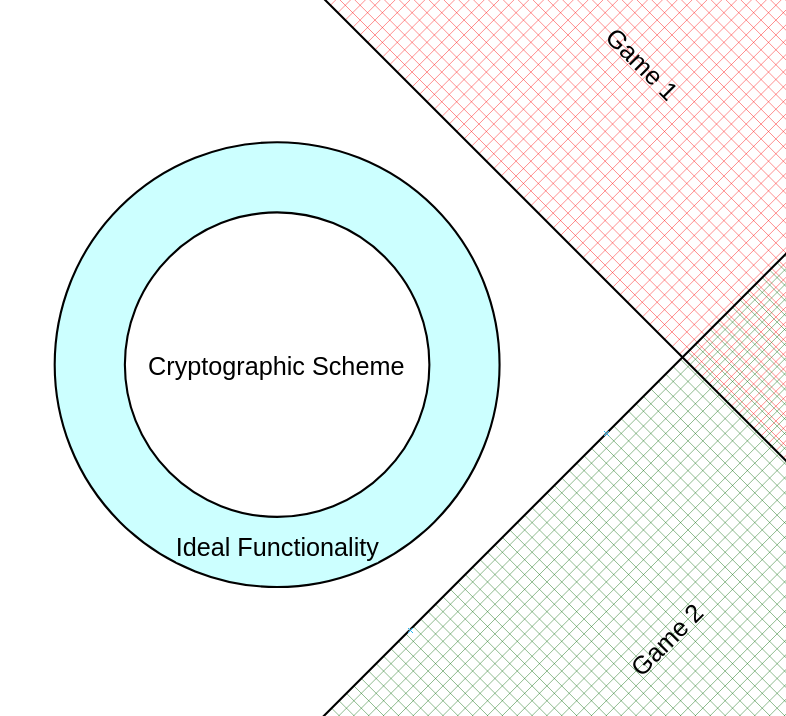
\includegraphics[width=10cm]{./01_body/images/simulation_vs_game_based_security.png}
\centering
\caption{Σχηματική αναπαράσταση Απόδειξης ασφάλειας μέσω παιχνιδιού και μέσω προσομοίωσης}
\label{fig:game_proof_vs_simulation_proof}
\end{figure}

